\documentclass[oneside]{book}
\usepackage{../Style/Master}
\usepackage{../Style/boxes}
\usepackage{../Style/Env}
\usepackage{../Style/DefNoteFact}
\usepackage{../Style/QnsProof}
\usepackage{../Style/Thms}
\usepackage{newpxtext, eulerpx}
\usepackage{bbding}
\begin{document}

\begin{titlepage}
    \frontmatter
    \begin{tikzpicture}[font=\sffamily,remember picture,overlay]
        \node[fill=Dandelion,anchor=north, minimum width=\paperwidth, minimum height=2cm] (names)
     at ([yshift=0]current page.north) {
      \begin{tabular}{c}
          \\
          \color{blue} {\fontsize{24.88pt}{65pt}\selectfont A-Levels Physics Notes}\\[2mm]
          \Large \color{blue}{By Grass}\\
          \color{blue} {\fontsize{10pt}{10pt}\selectfont Licensed under the GNU General Public License v3.0}\\
      \end{tabular}
      };
    \end{tikzpicture}

\begingroup
\let\clearpage\relax
\vspace{2cm}
\tableofcontents
\endgroup
\mainmatter
\end{titlepage}

\raggedright
\chapter{Kinematics}
\begin{center}
    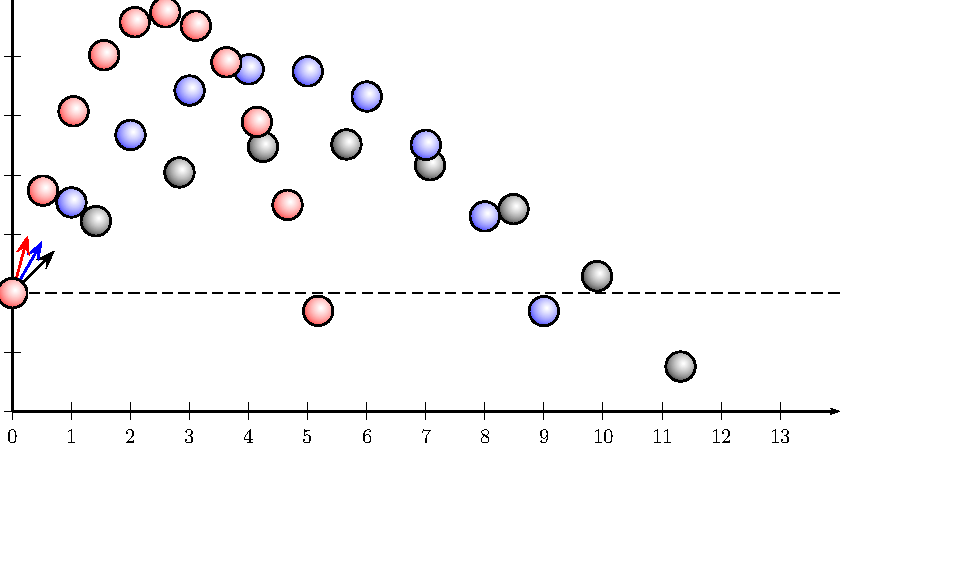
\includegraphics[width=\textwidth]{../images/Kinematics/schieferWurf.pdf}
    \captionsetup{type=figure}
    \caption[figure]{\ref{Projectile motion} Parabolic path travelled by balls thrown at varying angles.}
\end{center}
\begin{itemize}
    \item \textit{Distance} is defined as the total length of \emph{path} travelled.
    \item \textit{Velocity} is defined as the rate of change of displacement.
    \item \textit{Acceleration} is defined as the rate of change of velocity.
\end{itemize}
\chapter{Dynamics}
\begin{itemize}
    \item \textit{Newton's First Law of Motion} states that an object at rest will remain at rest and an object in motion will remain in motion at constant velocity in a straight line in the absence of an \emph{external} resultant force.
    \item The \textit{linear momentum} of a body is the product of its mass and velocity. The linear momentum is in the \emph{same direction} as it velocity.
    \item \textit{Newton's Second Law of Motion} states that the rate of change of momentum of a body is directly proportional to the resultant force acting on the body and occurs \emph{in the direction} of the resultant force.
    \item \textit{Newton's Third Law of Motion} states that if body A exerts a force on body B, then body B exerts a force of the \emph{same type} that is equal in magnitude and opposite in direction on body A.
    \item \textit{Impulse} is defined as the product of \emph{average} force acting on an object and the time for which the force acts.
    \item The \textit{Principle of Conservation of Linear Momentum} states that the total momentum of a system remains constant provided no \emph{external} resultant force acts on the system.
\end{itemize}
\chapter{Forces}
\begin{center}
    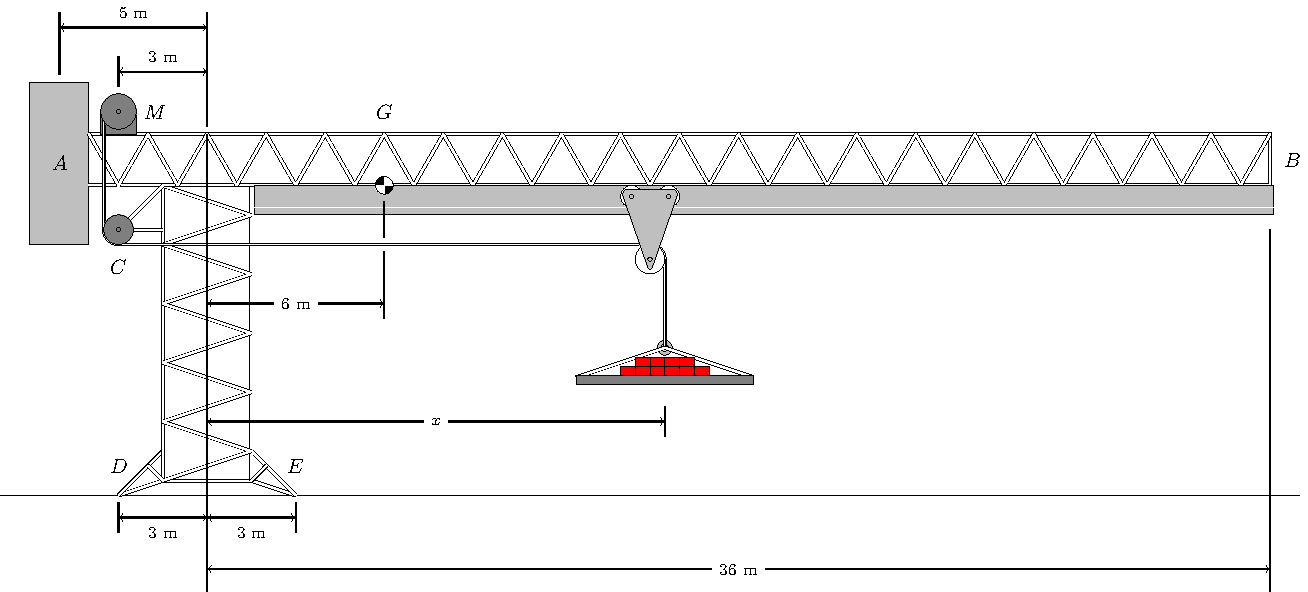
\includegraphics[width=\textwidth,page=1]{../images/Crane/Crane.pdf}
    \captionsetup{type=figure}
    \caption[figure]{\ref{Crane} Forces acting on a crane.}
\end{center}
\begin{itemize}
    \item \textit{Hooke's Law} states that the force is directly proportional to the extension in a material if its \emph{limit of proportionality} is not exceeded.
    \item The \textit{center of gravity} of an object is the point at which the entire weight of a body may be considered to act.
    \item The \textit{moment} of a force is equal to the product of the force and the \emph{perpendicular} distance of the \emph{line of action} of the force from the pivot. It is also the turning effect of a force.
    \item \textit{Torque of a couple} is defined as the product of one of the forces and the \emph{perpendicular} distance between the \emph{lines of action} of the forces.
    \item The \textit{Principle of Moments} states that if a body is in equilibrium, the sum of all the clockwise moments about \emph{any axis} must be equal to the sum of anticlockwise moments about the \emph{same axis}.
    \item \textit{Density} is defined as the mass per unit volume of a substance.
    \item \textit{Pressure} is defined as force per unit area, where the force is \emph{acting perpendicularly} to the area.
    \item Deriving \(p=\rho gh\):
    \begin{enumerate}
        \item Consider a point at a depth \(h\) below the surface of a liquid of density \(\rho\). 
        \item The force \(F\) acting perpendicularly on a surface area \(A\) at depth \(h\) is due to the weight of the liquid column above \(A\) to give pressure \(p\). Thus, \(p=\frac{F}{A}=\frac{mg}{A}=\frac{\rho Ah}{g}=\rho gh\).
    \end{enumerate}
    \item \textit{Upthrust} is the upward force exerted by a fluid on a body immersed in the fluid (due to pressure difference in the fluid).
    \item \textit{The origin of upthrust:} Upthrust is a result of the pressure difference between top and bottom surfaces of the body, resulting in a net upwards force being exerted on the body by the third medium in which the body is located.
    \item \textit{Archimedes' Principle} states that when a body is totally or partially immersed in a fluid, it experiences an upward force (upthrust) equal to the weight of fluid displaced.
    \item \textit{The Principle of Floatation} states that, for any object floating in \emph{equilibrium}, the upthrust is equal to the weight of the object.
\end{itemize}
\chapter{Work, Energy, and Power}
\begin{itemize}
    \item \textit{Work done} is defined as the product of a force and the displacement in the direction of the force.
    \item \textit{One joule of work} is defined as the work done by a force of 1 Newton when its \emph{point of application} moves through a distance of 1 metre in the direction of the force.
    \item \textit{Energy} is defined as the ability to do work.
    \item \textit{The Principle of Conservation of Energy} states that energy can neither be created or destroyed in \emph{any process}. It can be transformed from one form to another, and transferred from one body to another.
    \item Deriving \(E_k=\frac{1}{2}mv^2\): 
    \begin{enumerate}
        \item Consider a constant horizontal applied force \(F\) acting on an object of mass \(m\) travelling with initial velocity \(u\) to reach a final velocity \(v\) over a displacement \(s\). 
        \item For uniform acceleration, \(v^2=u^2+2as\) so \(as=\frac{1}{2}(v^2-u^2)\). Combined with Newton's Second Law, \(W=Fs=mas=\frac{1}{2}mv^2-\frac{1}{2}mu^2\). When the object starts from rest, \(u=0\). 
        \item By conservation of energy,\emph{ the work done by force \(F\) must be converted into the kinetic energy \(E_k\) of the object}. Hence, \(E_k=W=\frac{1}{2}mv^2-\frac{1}{2}m(0)^2=\frac{1}{2}mv^2\).
    \end{enumerate}
    \item The \textit{Work-Energy Theorem} states that the net work done by \emph{external} forces acting on a particle is equal to the change in kinetic energy of the particle.
    \item Deriving \(E_p=mgh\):
    \begin{enumerate}
        \item Consider an object from the Earth's surface --- which is taken as the reference for zero gravitational potential energy --- raised up by a \emph{constant force \(F\) equal to and opposite to the weight \(mg\)} of the object such that the object moves up at \emph{constant velocity} to a height \(h_2\). 
        \item Thus, the object moves at constant speed so \(\Delta E_k=0\). Therefore, 
        \begin{align*}
            \Delta E_p&= W\\
            E_p-0&=Fs\\
            E_p&=mgh.
        \end{align*}
        Where \(E_p\) is the gravitational potential energy at height \(h\) above the Earth's surface.
    \end{enumerate}
    \item Know how to \(\Delta E_p=\frac{1}{2}kx^2\) from area under graph.
    \item \textit{Power} is defined as the rate of doing work.
    \item Derive \(P=Fv\): \(P=\frac{\text{d}W}{\text{d}t}=\frac{F\text{d}s}{\text{d}t}=Fv\).
\end{itemize}
\chapter{Temperature and Ideal Gases}
\begin{itemize}
    \item The \textit{Zeroth Law of Thermodynamics} If bodies \(A\) and \(B\) are separately in thermal equilibrium with body \(C\), then bodies \(A\) and \(B\) are in thermal equilibrium with each other.
    \item \textit{One mole} is defined as the amount of substance that contains as many elementary particles as there are atoms in 0.012kg of carbon-12.
    \item \textit{Avogadro's Constant \(N_A\)} is the number of atoms in 0.012kg of carbon-12.
    \item ~\\[-3mm]
    \begin{tabular}{|Sc|Sl|}
        \hline
        & Assumptions of the Kinetic Theory of Gases\\
        \hline
        \textbf{M} & 
        \begin{tabular}{@{}Sl@{}}
            The molecules of the gas are in \emph{rapid} and \emph{random} motion.
          \end{tabular}\\
        \hline
        \textbf{A} & 
        \begin{tabular}{@{}Sl@{}}
            There are \emph{no intermolecular} attractive forces.
        \end{tabular}\\
        \hline
        \textbf{N} & 
        \begin{tabular}{@{}Sl@{}}
        Any gas consists of a \emph{very large number} of molecules.
        \end{tabular}\\
        \hline
        \textbf{T} & 
        \begin{tabular}{@{}Sl@{}}
        The duration of collisions is negligible compared\\ to the time interval between collisions.
        \end{tabular}\\
        \hline
        \textbf{E} & 
        \begin{tabular}{@{}Sl@{}}
        The collisions between gas molecules, and between\\ gas molecules and the container walls are \emph{perfectly elastic}.
        \end{tabular}\\
        \hline
        \textbf{V} & 
        \begin{tabular}{@{}Sl@{}}
        The volume of the gas molecules themselves is negligible \\compared to the volume of the container.
        \end{tabular}\\
        \hline
    \end{tabular}
    \item When do real gases behave like ideal gases: At high temperatures and low pressures.
    \item Deriving \(p=\frac{1}{3}\frac{Nm}{V}\langle c^2 \rangle\):
    \begin{enumerate}
        \item Consider a cubic container of side \(l\) containing \(N\) molecules, each of mass m.
        \item Change in momentum due to \emph{elastic} collision between wall and molecule\(\text{}=2mc_x\)
        \item Time interval between collisions, \(\Delta t=\frac{2l}{c_x}\).
        \item By Newton's 2nd Law, \(F=\frac{2mc_x}{\frac{2l}{c_x}}=\frac{mc_x^2}{l}\).
        \item Since \(A=l^2\), Pressure due to 1 particle, \(p=\frac{mc_x^2}{l^3}=\frac{mc_x^2}{V}\).
        \item Pressure due to \(N\) particles, \(p_N=\frac{Nmc_x^2}{V}\).
        \item By Pythagoras'Theorem, \(c^2=c_x^2+c_y^2+c_z^2\). The average speed in the \(x\), \(y\), and \(z\) directions can be taken to be \(c_x=c_y=c_z\) so \(c^2=3c_x^2\). Now, \(p_N=\frac{Nm\langle \frac{1}{3}c^2\rangle}{V}=\frac{1}{3}\frac{Nm\langle c^2 \rangle}{V}\).
    \end{enumerate}
\end{itemize}
\chapter{First Law of Thermodynamics}
\begin{itemize}
    \item The \textit{heat capacity} of a body is defined as the amount of thermal energy required to raise its temperature by one Kelvin / degree Celsius.
    \item The specific \textit{heat capacity} of a body is defined as the amount of thermal energy required to raise the temperature of one unit mass of the substance by one Kelvin / degree Celsius.
    \item The \textit{specific latent heat} of a body is defined as the thermal energy required to change \emph{phase} of one unit mass of a substance, \emph{without a change in temperature}.
    \item \textit{Internal energy} of a system is a sum of \emph{random distribution} of kinetic and potential energy \emph{associated with the molecules} of the system.
    \item The \textit{First Law of Thermodynamics} states that the \emph{increase} in internal energy of a closed system is the \emph{sum} of heat \emph{supplied} to the system and the work done \emph{on} the system. 
\end{itemize}
\chapter{Circular Motion}
\begin{itemize}
    \item \textit{Angular displacement} is the angle through which an object turns \emph{with respect to the center} of the circular path.
    \item \textit{The radian} is defined as the angle \emph{subtended} at the \emph{center} of a circle by an \emph{arc} of length equal to the radius of the circle. 
    \item \textit{Angular velocity} is the rate of change of angular displacement.
\end{itemize}
\begin{itemize}[label=\(\square\)]
    \item \begin{tabular}{|Sc|Sc|Sc|Sc|Sc|}
        \hline
            \(\begin{aligned}
                \omega=\frac{2\pi}{T}=2\pi f
            \end{aligned}\)&
            \(\begin{aligned}
                v=r\omega
            \end{aligned}\)&
            \(\begin{aligned}
                a_c=\frac{v^2}{r}=r\omega^2=v\omega
            \end{aligned}\)&
            \(\begin{aligned}
                F_c=ma_c
            \end{aligned}\)
        \\
        \hline
    \end{tabular}
    \item Common formulae: \(\theta=\tan^{-1}\left(\frac{v^2}{rg}\right)\), \(v=\sqrt{rg}\).
    \item Water in bucket at top position: \(F_c=N+W\) (where \(N\geq 0\)) so \(\omega>\sqrt{\frac{g}{r}}\).
    \item Need to write ``Centripetal force is provided by \underline{\hspace{1cm}}'' 
\end{itemize}
\chapter{Gravitational Fields}
\begin{itemize}
    \item \textit{Newton's Law of Gravitation} states that the force of attraction between any two point masses is directly proportional to the product of their masses and inversely proportional to the square of their separation.
    \item A \textit{gravitational field} is a region in space where mass experiences a gravitational force acting on it.
    \item Gravitational field strength at a point is defined as the gravitational force per unit mass acting on a small mass placed at that point
    \item The \textit{gravitational potential energy} of a mass at a point is defined as the work done by an \emph{external agent} in bringing the mass \emph{from infinity} to that point (without any net change in kinetic energy).
    \item \textit{Gravitational potential} at a point is defined as the work done per unit mass by an \emph{external agent} in bringing a mass \emph{from infinity} to that point (without a change in kinetic energy).
    \item Escape velocity is the \emph{minimum} velocity a mass needs to be projected from the \emph{surface} of the moon in order to have sufficient kinetic energy to overcome the gravitational field it experiences and \emph{move to infinity}.
    \item Escape velocity \(v_\text{min}=\sqrt{\frac{2GM}{r}}\) (where Min \(E_k\) needed is the gain in \(E_p\) to reach infinity).
\end{itemize}
\begin{itemize}[label=\(\square\)]
    \item \[
\begin{tikzcd}[row sep=large, column sep=large]
     U_G=-\frac{GMm}{r} \arrow{r}{-\frac{\text{d}}{\text{d}r}} \arrow[swap]{d}{\frac{1}{m}} & F_G=-\frac{GMm}{r^2} \arrow[swap]{d}{\frac{1}{m}} \\
     \phi=-\frac{GM}{r} \arrow{r}{-\frac{\text{d}}{\text{d}r}} & g=-\frac{GM}{r^2}\\
\end{tikzcd}
\]
\item \(U_G=m\phi\) \& \(\Delta U_G=m\Delta\phi\).
\item \(U_G\) is negative because infinity is taken as the reference point for zero potential energy. The work done against gravitational force in bringing a mass from infinity to that point is negative.
\item Gravitational force provides the centripetal force:
\begin{align*}
    F_G&=F_c\\
    \frac{GMm}{r^2}&=mr\omega^2=mr\left(\frac{2\pi}{T}\right)^2\\
    T^2&=\frac{4\pi^2}{GM}r^3\\
    T^2 &\propto r^3
\end{align*}
\item Gravitational force provides the centripetal force:
\begin{alignat*}{2}
    && F_G&=F_c\\
    &\text{For \(A\):}& \hspace{1cm} \frac{Gm_Am_B}{(r_A+r_B)^2}&=m_Ar_A\omega^2\\
    &\text{For \(B\):}& \frac{Gm_Am_B}{(r_A+r_B)^2}&=m_Br_B\omega^2
\end{alignat*}
The center of mass of the system is at point \(P\) where 
\[m_Ar_A=m_Br_B\]
such that both stars have the same angular velocity \(\omega\).
\item For binary star systems, notice that \emph{orbital radius is replaced by the stars' separation}:
\begin{align*}
    m_Ar_A&=m_Br_B& && \frac{Gm_Am_B}{(r_A+r_B)^2}&=m_Br_B\omega^2\\
    r_A+r_B&=\frac{m_B}{m_A}r_B+r_B& &\text{so}& &=\frac{m_Am_B}{m_A+m_B}(r_A+r_B)\omega^2\\
    r_B&=\frac{m_A}{m_A+m_B}(r_A+r_B)& && &\\
\end{align*}
So, rearranging, we have
\[\omega^2=\frac{G(m_A+m_B)}{(r_A+r_B)^3}=\frac{Gm_A}{r_B(r_A+r_B)^2} \qquad\text{and}\qquad T^2=\frac{4\pi^2}{G(m_A+m_B)}(r_A+r_B)^3.\]
\item Geostationary orbit facts:
\begin{enumerate}
    \item Only one such orbit at a \emph{fixed} distance of \(4.2\times10^7\text{m}\) from Earth's center,
    \item Orbital period of 24 hours,
    \item Satellite's plane of orbit coincides with the equatorial plane of the Earth,
    \item Orbits West to East (in the same direction as Earth's rotation). 
\end{enumerate}
\item Equipotential lines are not equally spaced because the gravitational field strength is not constant but decreases as one goes away from the Earth.
\item Assumptions made in the theory (e.g. in deriving \(g=-\frac{GM}{r^2}\)):
\begin{enumerate}
    \item The bodies are separated by distances so large they can be considered as point particles (i.e. separation >> radius).
    \item The bodies are homogenous spheres (constant density throughout the sphere).
    \item The bodies have masses distributed symmetrically around the center in uniform layers.
    \item In the absence of other masses.
\end{enumerate}
\end{itemize}
\begin{center}
    \includegraphics[width=\textwidth]{../images/2024-Eclipse-Map-(cit\_).png}
    \captionsetup{type=figure}
    \caption[figure]{\ref{2024 Eclipse Map} Forces acting on a crane.}
\end{center}
\emph{Note.} According to the author of this image, when compared to their above prediction,
\begin{enumerate}
    \item The duration of eclipse at greatest eclipse is 2 seconds shorter.
    \item The moments of contact are a couple seconds off.
\end{enumerate}
\chapter{Oscillations}
\begin{center}
    \includegraphics[width=0.25\textwidth,page=20]{../images/SHM/SHMCropped.pdf}
    \captionsetup{type=figure}
    \caption[figure]{\ref{Simple harmonic motion} Simple harmonic motion.}
\end{center}
\begin{itemize}
    \item \textit{Simple harmonic motion} is defined as the motion of a body whose acceleration is directly proportional to its displacement from a fixed point (equilibrium position) and is always directed towards that fixed point.
    \item A \textit{freely oscillating} system oscillates at its own \textit{natural frequency} without \emph{external} influences other than the \emph{initial impulse when displaced} from its equilibrium position, with \emph{no dissipation} of energy.
    \item \textit{Damped oscillations} are oscillations in which the amplitude diminishes with time as a result of \emph{dissipative forces} that reduce the total energy of the oscillations.
    \item A system is in \textit{forced oscillations} when it is forced to oscillate at a frequency other than the natural frequency by a \emph{periodic external} force.
    \item \textit{Resonance} is a phenomenon that occurs when the frequency at which an object is being made to vibrate (the forced frequency of vibration) is equal equal to its natural frequency of vibration.
\end{itemize}
\begin{itemize}[label=\(\square\)]
    \item \begin{tabular}{|Sc|Sc|Sc|Sc|Sc|}
        \hline
        \multirow{2}{*}[-1em]{\(\begin{aligned}
            v=\pm \omega \sqrt{x_0^2-x^2}
        \end{aligned}\)}&\multirow{2}{*}[-1em]{\(\begin{aligned}
            a=-\omega^2x
        \end{aligned}\)}& Spring-Mass & Pendulum\\
            &
            &
            \(\begin{aligned}
                T=2\pi\sqrt{\frac{m}{k}}
            \end{aligned}\)&
            \(\begin{aligned}
                T=2\pi\sqrt{\frac{l}{g}}
            \end{aligned}\)
        \\
        \hline
    \end{tabular}
    \item \begin{tabular}{|Sc|Sc|Sc|Sc|}
        \hline
        &
    \(\begin{aligned}
        E_k
    \end{aligned}\)&
    \(\begin{aligned}
        E_p
    \end{aligned}\)&
    \(\begin{aligned}
            E_T
    \end{aligned}\)\\
    \hline
        \(\begin{aligned}
            t
        \end{aligned}\)&
        \(\begin{aligned}
            \frac{1}{2}m\omega^2x_0^2\cos^2(\omega t)
        \end{aligned}\)&
        \(\begin{aligned}
            \frac{1}{2}m\omega^2x_0^2\sin^2(\omega t)
        \end{aligned}\)&
        \(\begin{aligned}
            \frac{1}{2}m\omega^2x_0^2
        \end{aligned}\)\\
        \hline
        \(\begin{aligned}
            m
        \end{aligned}\)&
        \(\begin{aligned}
            \frac{1}{2}m\omega^2(x_0^2-x^2)
        \end{aligned}\)&
        \(\begin{aligned}
            \frac{1}{2}m\omega^2x^2
        \end{aligned}\)&
        \(\begin{aligned}
            \frac{1}{2}m\omega^2x_0^2
        \end{aligned}\)\\
        \hline
    \end{tabular}
    \item Simple pendulums and mass spring systems can be approximated to be SHM when the angle of oscillation (\(\leq 20^\circ\)) and oscillation amplitude are small, respectively.
    \item \begin{tabular}{|Sc|Sc|Sc|Sc|}
        \hline
        & In Phase & Antiphase & Out of Phase\\
        \hline
        \(\Delta \phi\)/rad & 0 & \(\pi\) & nonzero
        \\
        \hline
    \end{tabular}
    \item When damping increases:
    \begin{itemize}[label=\(\circ\)]
        \item Amplitude at \emph{all} frequencies decreases.
        \item (Resonance) frequency at max amplitude shifts gradually to lower frequencies.
        \item Peak (max amplitude) becomes flatter.
    \end{itemize}
\end{itemize}
\chapter{Wave Motion}
\begin{itemize}
    \item A \textit{progressive} wave is a wave in which \emph{energy is carried} from one point to another by means of \emph{vibrations or oscillations} within the wave. Particles within the wave are \emph{not transported along} the wave.
    \item A \textit{phase} is an angle which gives a measure of the \emph{fraction of a cycle} that has been \emph{completed} by an oscillating particle or by a wave.
    \item \emph{Intensity} of a wave is the wave energy incident per unit time per unit area \emph{normal} to the wave.
    \item \textit{Polarisation} of a wave refers to the \emph{confinement} of oscillations in \emph{only} one plane. The plane of oscillations is \emph{parallel} to the direction of energy transfer.  
    \item Malus' Law states that the intensity of a beam of \emph{plane polarised light} after passing through a rotatable polariser is directly proportional to the square of the cosine of the angle through which the polariser is rotated from the position that gives maximum intensity. (\(I=I_{\text{max}}\cos^2(\theta)\))
\end{itemize}
\begin{itemize}[label=\(\square\)]
    \item \begin{tabular}{|Sc|Sc|Sc|}
        \hline
        Phase Difference \(\Delta \phi\) & \(\frac{2\pi}{\lambda}\Delta x\) & \(\frac{2\pi}{T}\Delta t\)\\
        \hline
    \end{tabular}
    \item \begin{tabular}{|Sc|Sc|Sc|Sc|}
            \hline
            \multicolumn{4}{|Sc|}{Intensity}\\
            \hline
            \multirow{2}{*}{Amplitude} & \multicolumn{3}{Sc|}{Wave}\\
            \cline{2-4}
            & Spherical & Circular & Plane\\
            \hline
            \(I \propto A^2\) & \(I \propto \frac{1}{r^2}\) & \(I \propto \frac{1}{r}\) & \begin{minipage}{3cm}
                \vspace{1mm}\begin{center}
                    \(I\) is constant\\
                \tiny (No spreading of waves) \normalsize
                \end{center}
            \end{minipage}\\
            \hline
        \end{tabular}
        \item[\mbox{\FiveStarOpen}] When unpolarised light passes through a polariser, the average value of \(\cos^2(\theta)\) is \(\frac{1}{2}\) so \(I_\text{new}=\frac{1}{2}I_\text{max}\). 
\end{itemize}

\chapter{Superposition}
\begin{itemize}
    \item \emph{Principle of Superposition}: When two or more waves of the \emph{same type}, meet at \emph{a point in space}, the \emph{resultant displacement} of the waves at any point is the \emph{vector sum} of the \emph{displacements} due to \emph{each wave acting independently} at that point.
    \item \emph{Stationary waves} are waves whose \emph{waveforms does not advance} and there is \emph{no net translation of energy}. The \emph{amplitude} of the waves varies according to \emph{position} from zero at the nodes to a maximum at the antinodes.
    \item A stationary wave is formed when two \emph{progressive} waves
    \begin{enumerate}
        \item Having the \emph{same frequency} and \emph{same speed}
        \item Travel in \emph{opposite directions} towards each other
        \item Have \emph{similar amplitudes}
        \item Are unpolarised, or polarised along the same axis
        \item Are \emph{superposed} 
    \end{enumerate}
    \item \begin{tabular}{|Sc|Sc|Sc|}
        \hline
        \multirow{2}{*}{Properties} & \multicolumn{2}{Sc|}{Reflection Surface}\\
        \cline{2-3}
        & Loose End\footnotemark[1] & Fixed End\\
        \hline
        Allows for Oscillations? & Yes & No\\
        \hline
        Will Reflected Wave be Inverted (phase change of \(\pi\))? & No & Yes\\ 
        \hline
    \end{tabular}
    \footnotetext[1]{Particles of the wave can move about freely.}
    \item Characteristics of Stationary Waves:
    \begin{enumerate}
        \item Displacement node = Pressure antinode
        \item Displacement antinode = Pressure node
    \end{enumerate}
    \begin{longtable}{|Sc|Sc|Sc|}
        \hline
        Properties & Stationary Wave & Progressive Wave\\
        \hline
        Energy & No net transfer of energy & 
        \begin{minipage}{0.4\textwidth}
            Energy is transferred in the direction of propagation of the wave. 
        \end{minipage}\\
        \hline
        Phase & 
        \begin{minipage}{0.4\textwidth}
            \begin{itemize}[label=\(\square\)]
                \item Adjacent nodes: In phase
                \item Adjacent segments: Antiphase. \hyperlink{StationaryWavesPhase}{(Fig 12.1)}
            \end{itemize}
        \end{minipage} & 
        \begin{minipage}{0.4\textwidth}
            All points within one wavelength have different phases.
        \end{minipage}\\
        \hline
        Amplitude &
        \begin{minipage}{0.4\textwidth}
            Varies: 0 at nodes to max at antinodes.
        \end{minipage}
        &
        \begin{minipage}{0.4\textwidth}
            Same for all particles.
        \end{minipage}\\
        \hline
        Wavelength &
        \begin{minipage}{0.4\textwidth}
            Twice the distances between adjacent nodes or adjacent antinodes.
        \end{minipage} &
        \begin{minipage}{0.4\textwidth}
            Distance between adjacent in-phase particles. 
        \end{minipage}\\
        \hline
        Frequency &
        \multicolumn{2}{Sc|}{Same for all particles}\\
        \hline
        Nodes\footnotemark[2]/Antinodes\footnotemark[3] & \checkmark & \(\times\)\\
        \hline
    \end{longtable}
    \footnotetext[2]{At which particles don't oscillate/\(\text{amplitude}=0\).}
    \footnotetext[3]{At which particles have the largest amplitude.}
    \newpage
    \begin{center} \hypertarget{StationaryWavesPhase}{}
        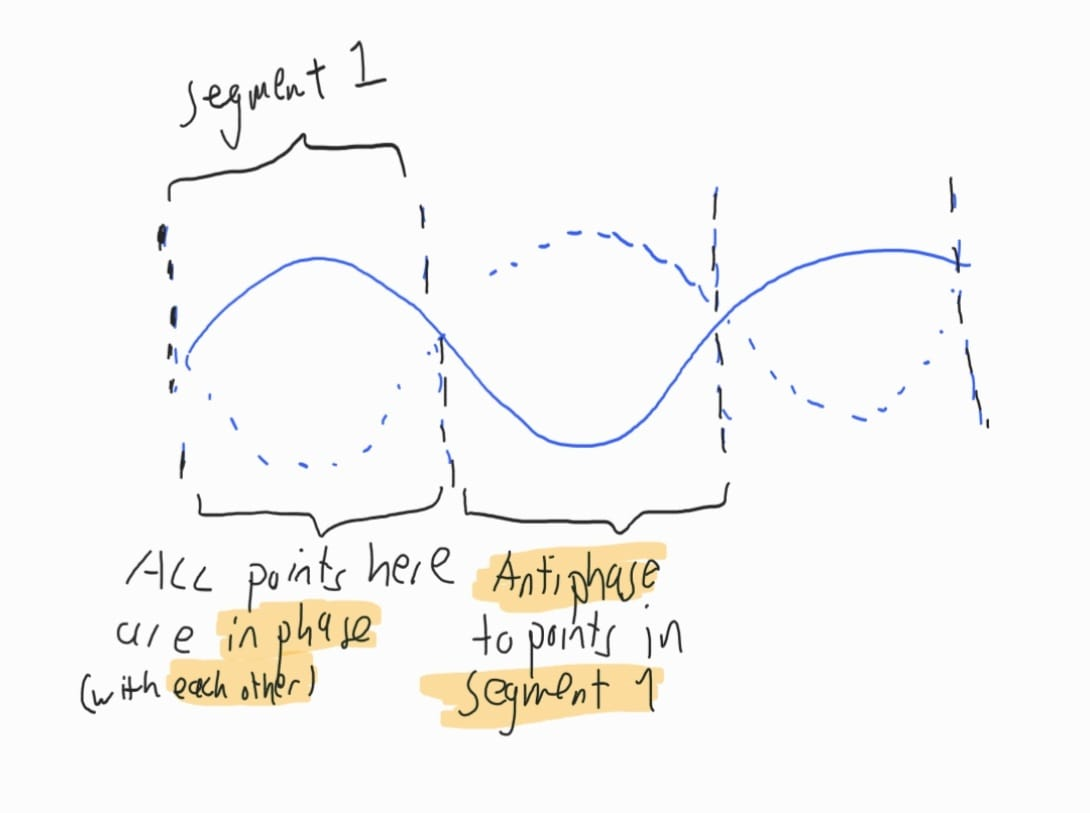
\includegraphics[scale=0.2]{../images/StationaryWavesPhase.jpg}
        \captionsetup{type=figure}
        \captionof{figure}{\ref{Me} Phases in stationary waves}
    \end{center}
    \resizebox{\textwidth}{!}{\begin{tabular}{|Sc|Sc|Sc|Sc|Sc|Sc|}
        \hline
        & \multicolumn{2}{Sc|}{Modes} & \multirow{2}{*}{Diagrams} & \multirow{2}{*}{Wavelength} & \multirow{2}{*}{Frequency}\\
        \cline{2-3}
        & Overtone & Harmonic &&&\\
        \hline
        Strings/Open Pipes & \multirow{2}{*}{\(n\)th} & \((n+1)\)th & \hyperlink{Fig 12.2}{12.2} \& \hyperlink{Fig 12.3}{12.3} & \(\lambda=\frac{2L}{n+1}\) & \(f=(n+1)\frac{v}{2L}\)\\
        \cline{1-1}
        \cline{3-6}
        Pipes Closed at One End & & \((2n+1)\)th & \hyperlink{Fig 12.4}{12.4} \& \hyperlink{Fig 12.5}{12.5} & \(\lambda=\frac{4L}{2n+1}\) & \(f=(2n+1)\frac{v}{4L}\)\\
        \hline
    \end{tabular}}
    \begin{minipage}{0.3\textwidth}
        \begin{center}
            \hypertarget{Fig 12.2}{}
            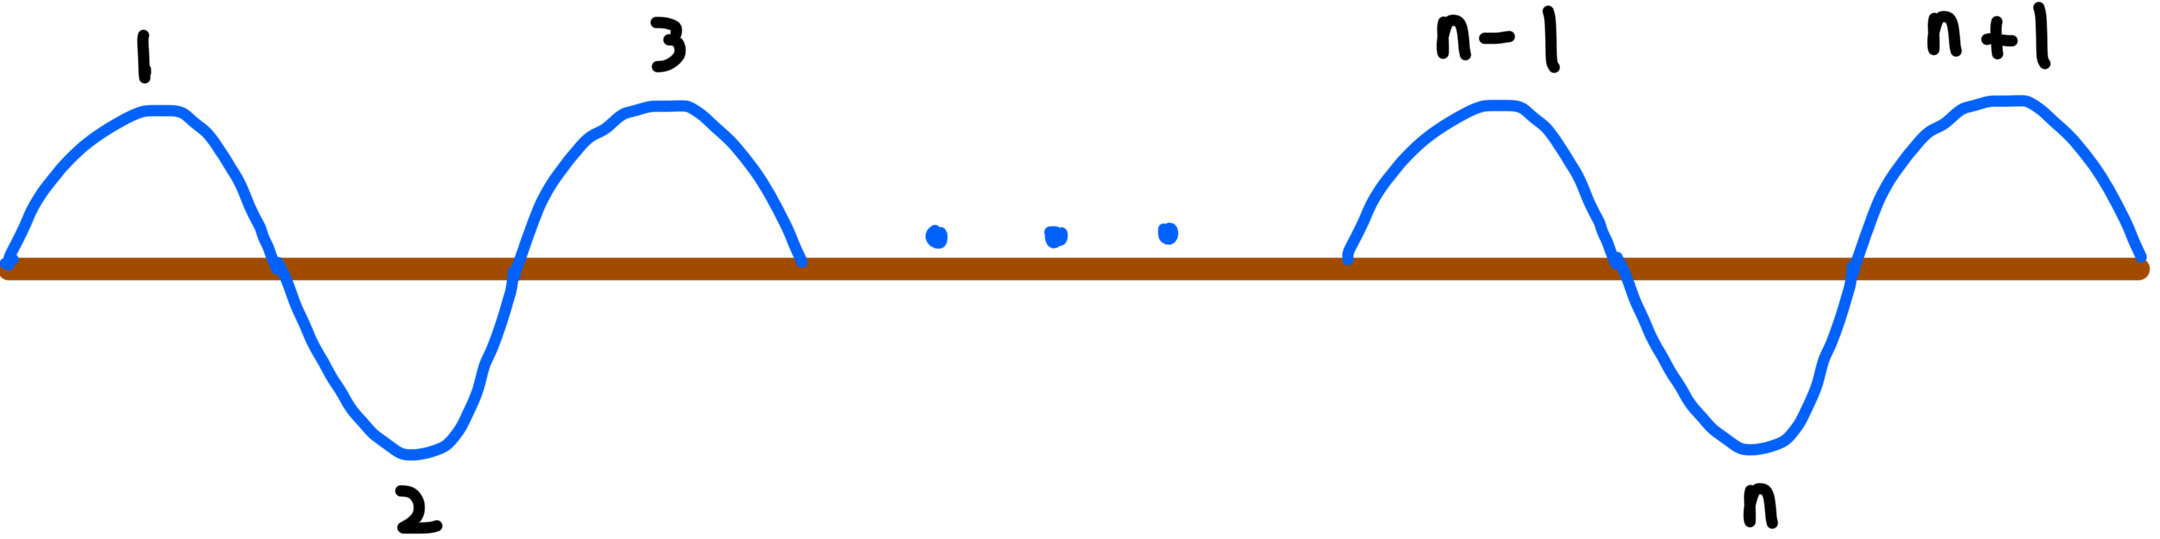
\includegraphics[scale=0.1]{../images/StringStatWaves.jpg}
            \captionsetup{type=figure}
            \captionof{figure}{\ref{RVHS} String.}
        \end{center}
    \end{minipage}
    \begin{minipage}{0.3\textwidth}
        \begin{center}
            \hypertarget{Fig 12.3}{}
            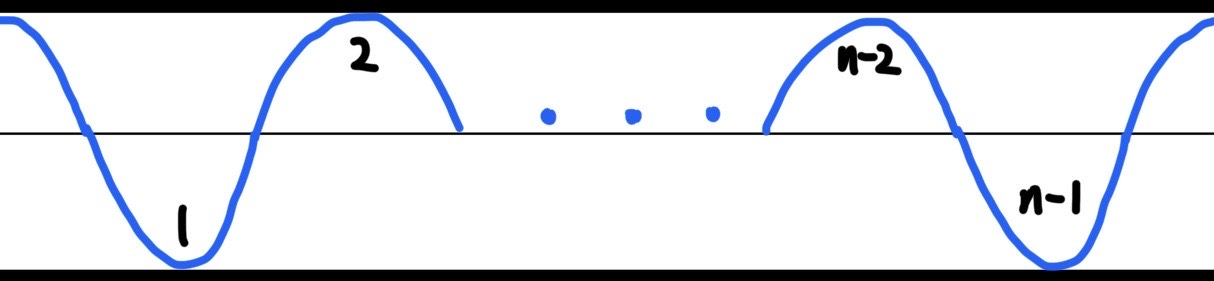
\includegraphics[scale=0.1]{../images/Open Pipe.jpg}
            \captionsetup{type=figure}
            \captionof{figure}{\ref{RVHS} Open pipe.}
        \end{center}
    \end{minipage}
    \begin{minipage}{0.3\textwidth}
        \vspace{7mm}
        \begin{center}
            \hypertarget{Fig 12.4}{}
            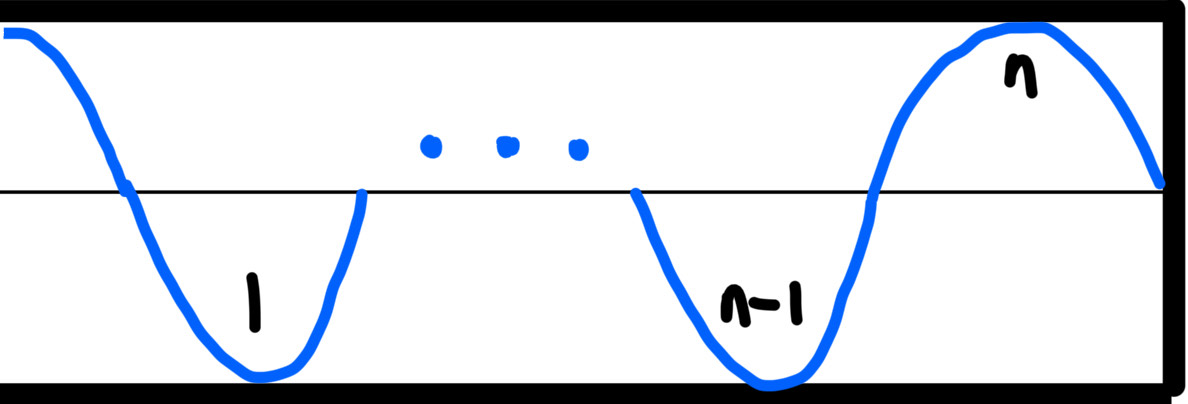
\includegraphics[scale=0.1]{../images/Pipe Closed at One End.jpg}
            \captionsetup{type=figure}
            \captionof{figure}{\ref{RVHS} Pipe closed at one end}
        \end{center}
    \end{minipage}
    \begin{center}
        \hypertarget{Fig 12.5}{}
        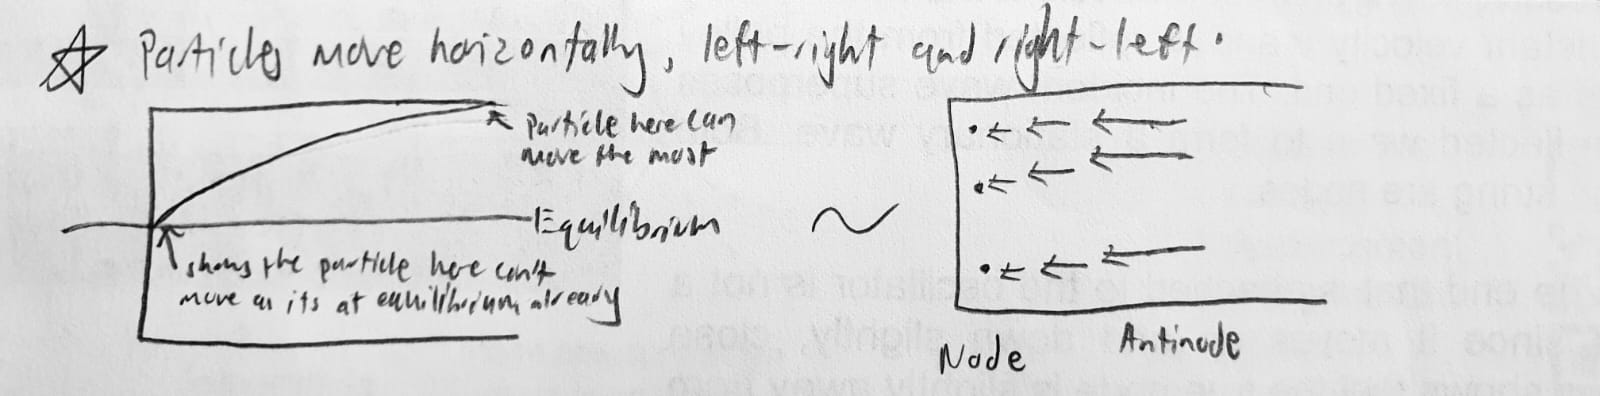
\includegraphics[scale=0.25]{../images/Pipe Closed At One End Movement.jpg}
        \captionsetup{type=figure}
        \captionof{figure}{Movement of particles in pipe.}
    \end{center}
    \setcounter{footnote}{1}
    \item Resonance length\footnote{End correction: Actual length of vibration is \(L+2c\) for open pipes, and \(L+c\) for closed pipes.} with pipes closed at one end 
    \[L=\frac{\lambda}{4}=\frac{v}{4f}.\]
    \begin{example}{}{}
        Explain, with reference to resonance, why the loudness of sound changes as the water level changes.
        \begin{enumerate}
            \item Natural frequency of vibration depends on length of air column.
            \item When fork frequency is equal to natural frequency/odd multiple of fundamental frequency, resonance occurs. There is maximum energy transfer and maximum amplitude of vibrations, leading to maximum loudness.
            \item When fork frequency is not equal to natural frequency, no resonance occurs and loudness drops.
        \end{enumerate}
    \end{example}
    \item If a tube achieves stationary waves at fundamental frequency \(f\), then reducing \(f\)/increasing \(\lambda\) will not result in stationary waves.
    \item \emph{Diffraction} is the \emph{bending or spreading out} of waves when they travel through a \emph{small opening} or when they pass round a \emph{small obstacle}.
    \item Large amount of diffraction occurs when the width of slit is about the same as the wavelength.
    \item The wavelength before and after diffraction should be around the same.
    \item Single Slit Diffraction: Let \(b\) be the slit width, and \(L\) the slit-screen distance.
    \begin{enumerate}
        \item For all nonzero integers \(m\), the angular positions \(\theta\) of the \(1 \leq m\)th order minima satisfies 
        \[\sin(\theta)=\frac{m\lambda}{b}.\] 
        \item Distance \(y_1\) of the first minima from either side of the central bright fringe is
        \[y_1=\frac{\lambda L}{b}.\]
    \end{enumerate}
    \begin{center}
        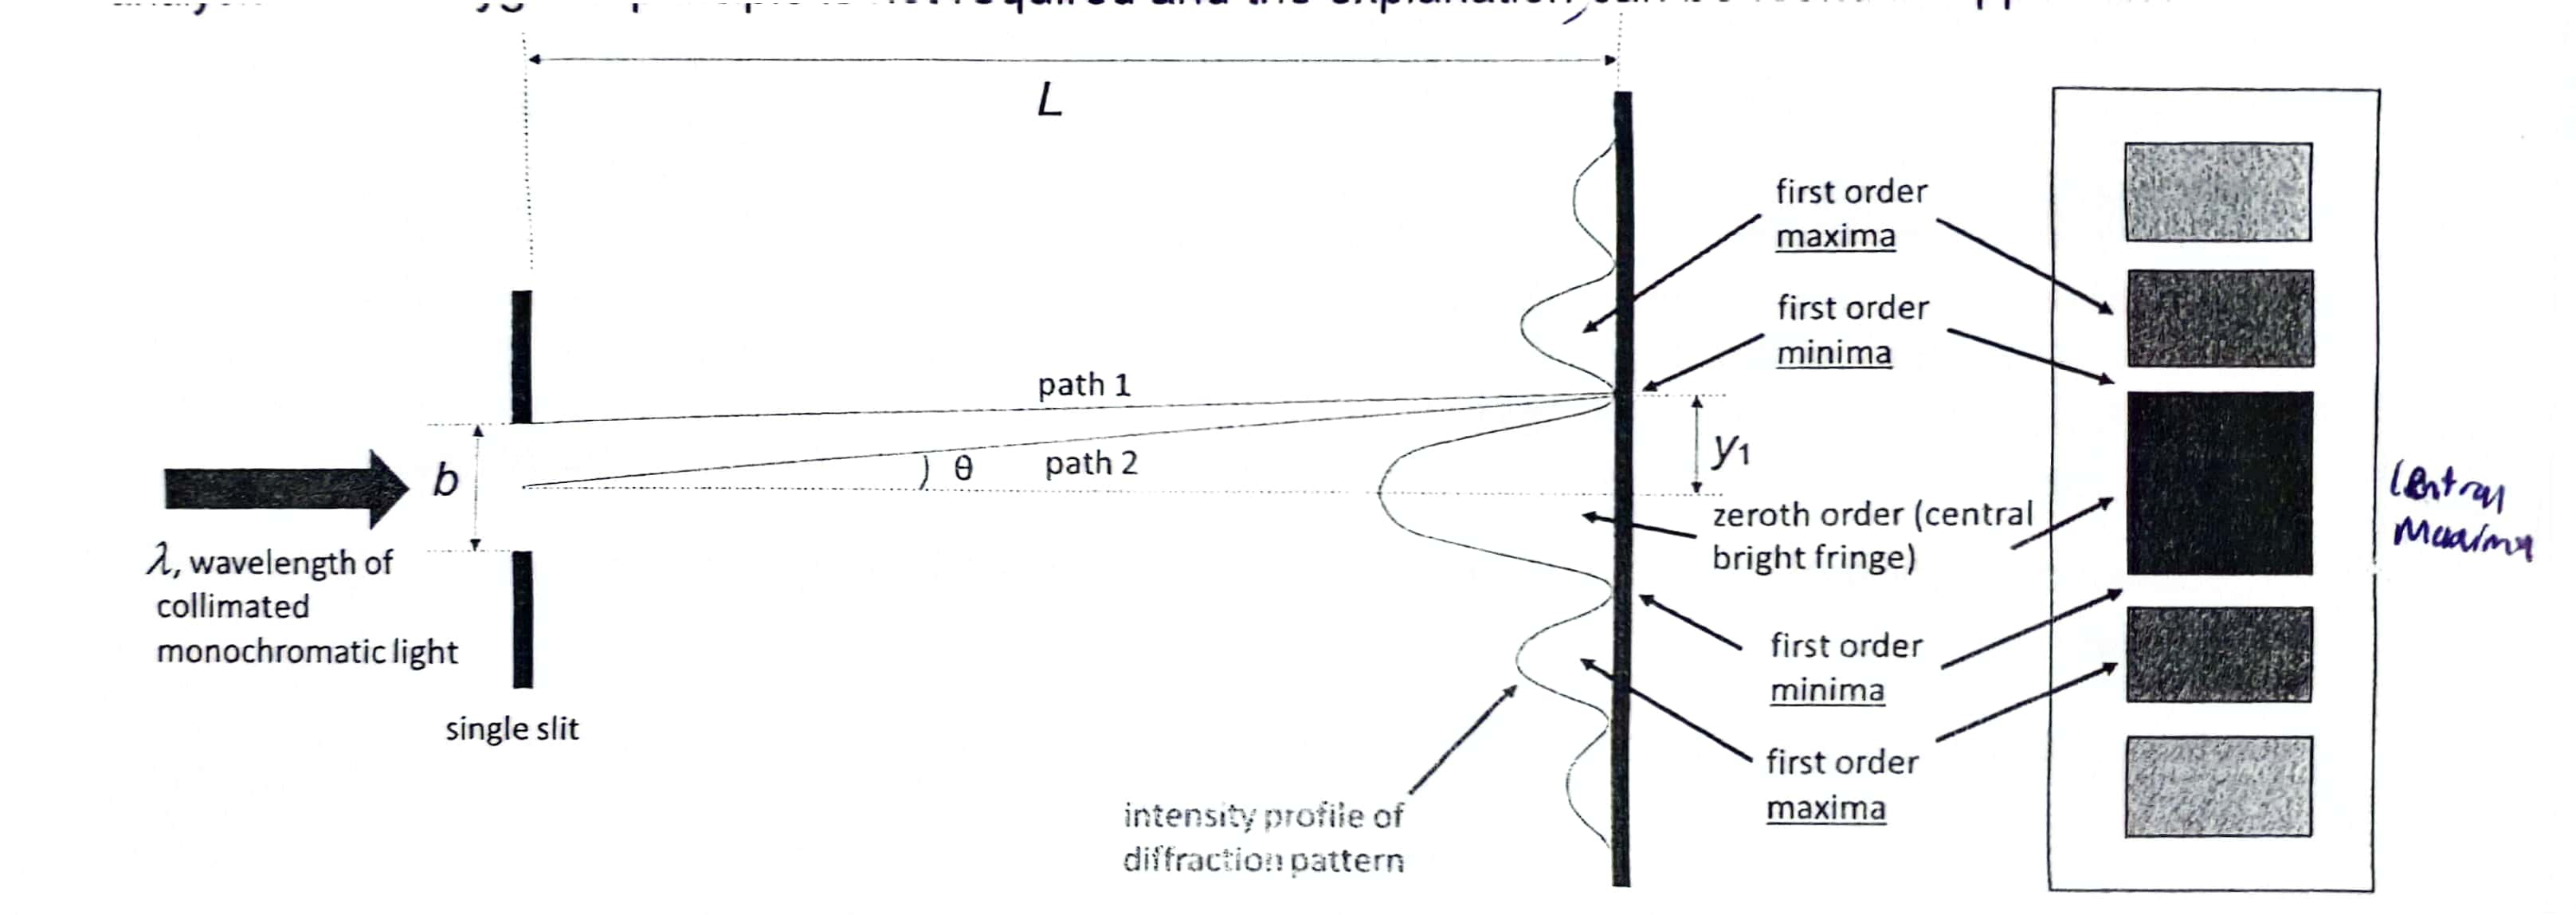
\includegraphics[scale=0.1]{../images/Single Slit Diffraction.jpg}
        \captionsetup{type=figure}
        \captionof{figure}{\ref{RVHS} Single slit diffraction.}
    \end{center}
    \item \emph{Circular} aperture: \(\theta \approx \frac{\lambda}{b}\).
    \item \emph{Rayleigh's Criterion} is the \emph{minimum separation} between two objects in order to be distinguished as two \emph{distinct} objects:
    \[\theta \approx \frac{\lambda}{b}.\]
    \item Sources are \emph{coherent} if they have a \emph{constant phase difference} with respect to time.
    \item \emph{Interference} is the \emph{superposing} of two or more waves to produce \emph{regions of maxima and minima} in space, according to the \emph{Principle of Superposition}.
    \item Conditions for an \emph{observable} interference pattern: 
    \begin{enumerate}
        \item The waves must \emph{overlap} to produce regions of maxima and minima.
        \item The \emph{sources} must be \emph{coherent}.
        \item The waves must have approximately the \emph{same amplitude}.
        \item The waves, if transverse, must be \emph{unpolarised} or have the \emph{same plane of polarisation}. 
    \end{enumerate}
    \item For \(n \in \mathbb{Z}^{+}_{0}\), representing the \(n\)th order max/min, we have 
    \resizebox{\textwidth}{!}{\begin{tabular}{|Sc|Sc|Sc|}
        \hline
        \multirow{2}{*}{Sources' Phase Difference} & \multicolumn{2}{Sc|}{Path Difference}\\
        \cline{2-3}
         & Constructive Interference (maxima) & Destructive Interference (minima)\\
        \hline 
        In phase & \(\Delta=n\lambda\) & \(\Delta=(n+1/2)\lambda\)\\
        \hline
        Out-of-phase & \(\Delta=(n+1/2)\lambda\) & \(\Delta=n\lambda\)\\
        \hline
    \end{tabular}}
    \item We always need to take the path difference starting from the actual source itself, even when the source travels through two slits onto a screen, for instance.
    \item Double-slits: For\footnote{Typical values: \(a \approx 0.5\)mm, \(D \approx 1\)m, and \(\lambda \approx 600\)nm. In any case, using the equation requires \(a<<D\).} a (\emph{center-to-center}) slit separation \(a\) and slit-screen distance \(D\), the fringe separation (between two adjacent minima, or two adjacent maxima) is
    \[x=\frac{\lambda D}{a}.\]
    \begin{center}
        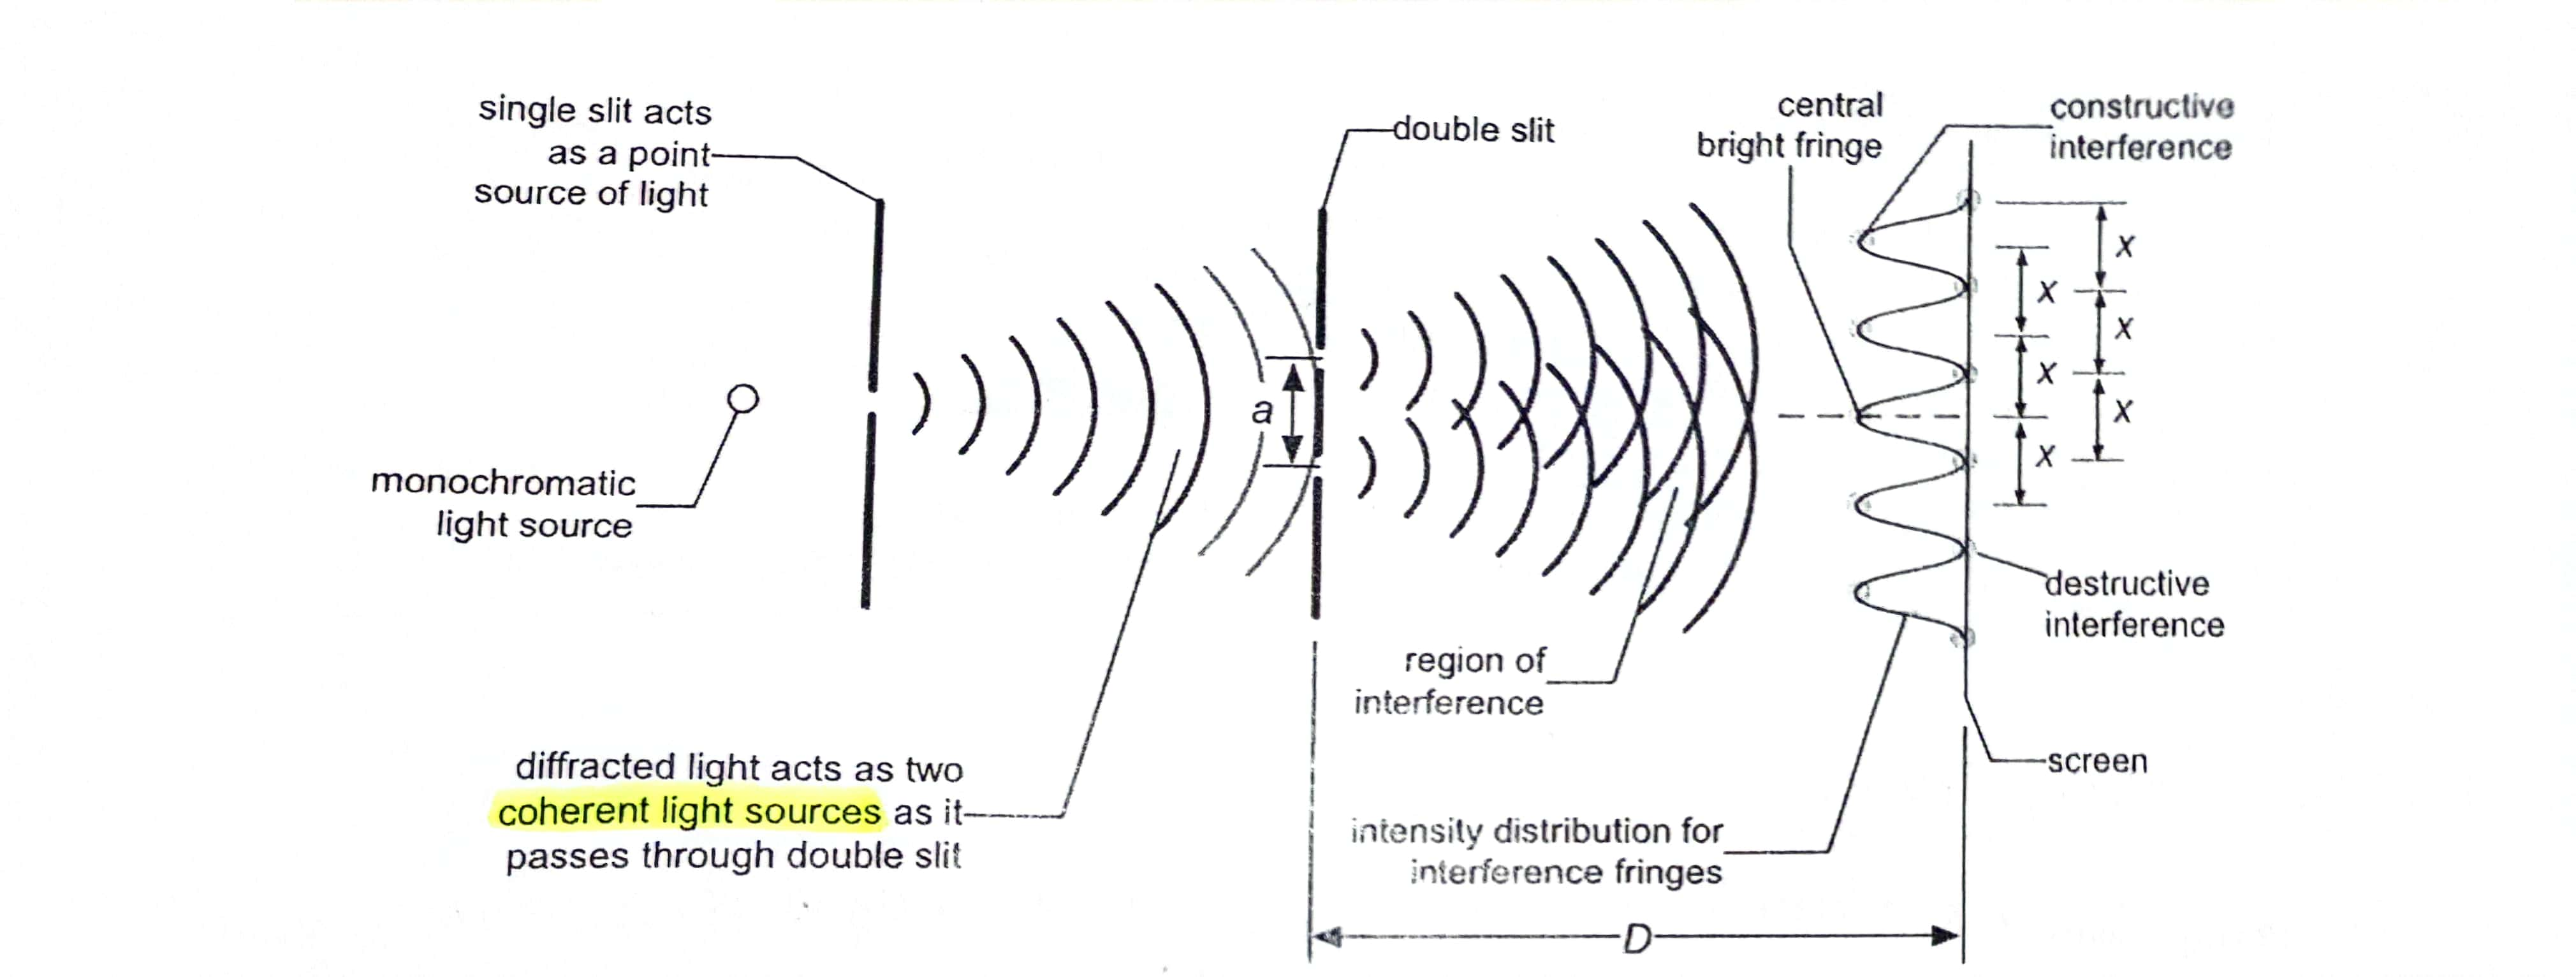
\includegraphics[scale=0.1]{../images/Double-Slit Diffraction.jpg}
        \captionsetup{type=figure}
        \captionof{figure}{\ref{RVHS} Double-slit diffraction.}
    \end{center}
    \setcounter{footnote}{4}
    \footnotetext{The intensity of the double-slit interference pattern is not constant because of single-slit diffraction effects.}
    \item Diffraction grating: For a slit-separation \(d\) and \(n \in \mathbb{Z}^{+}_{0}\), the angular positions for the \(n\)th order maxima satisfies
    \[d \sin(\theta_n)=n\lambda.\]
    \begin{center}
        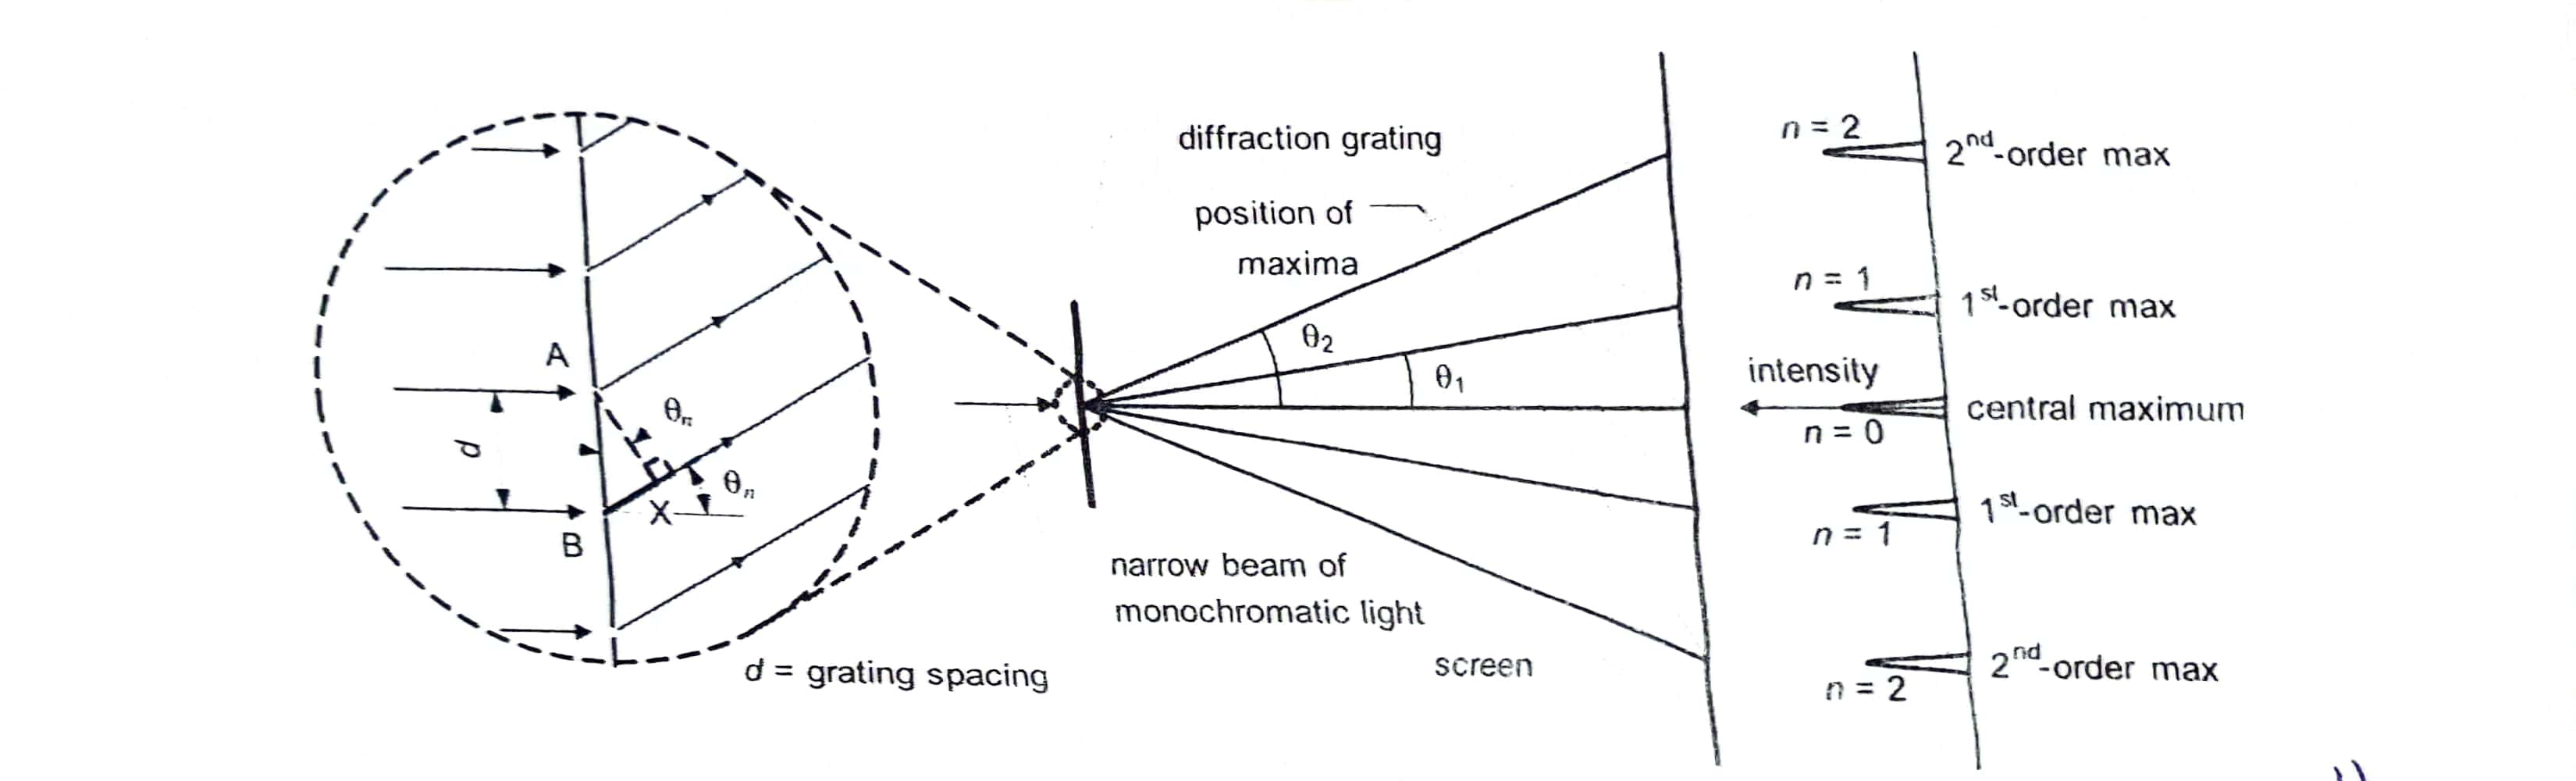
\includegraphics[scale=0.1]{../images/Diffraction Grating.jpg}
        \captionsetup{type=figure}
        \captionof{figure}{\ref{RVHS} Diffraction grating.}
    \end{center}
    \item Check answer: For visible light, \(400\text{nm} \leq \lambda \leq 700\text{nm}\).
    \item Total number of bright regions = 2\(\cdot\)highest order+1.
    \item When slit width is reduced, intensity is reduced.
    \item To calculate \emph{resultant intensity}, first take the sum of the amplitudes and use proportionality (\(I \propto A^2\)).  
    \item Every other line means half of the lines are covered.
    \begin{example}{}{}
        Describe and explain the appearance of the central fringe if the light is now replaced with white light.
    \begin{enumerate}
        \item The central bright fringe is generally white.
        \item The zeroth order fringes of all the wavelengths coincide at the center where the path difference from the two slits is zero for all wavelengths. The combined central fringes remains white.
        \item The sides of the central fringes are likely more reddish.
        \item  This is because the wider red fringe extends beyond the narrower blue fringe.
    \end{enumerate}
    \end{example}
\end{itemize}

\chapter{Currents of Electricity}
\begin{itemize}
    \item The \emph{number density} \(n\) is defined as the number of particles per unit volume.
    \item The \emph{drift velocity} \(v\) is the \emph{average} velocity at which \emph{charge carriers} move through a \emph{conductor} when there is \emph{electric current in the conductor}.
    \item Deriving the equation \(I=nAvq\):
    \begin{enumerate}
        \item Assume that the \emph{current is constant}. Then, \(I=\frac{Q}{t}\).
        \hspace*{0pt}\hfill \(\highlight[yellow]{[n]}\)
        \item Assume that there are \(N\) charge carriers passing through a cross-sectional area \(A\) in time \(t\), and that \emph{each} of them carries an \emph{identical amount of charge} \(q\). Then, the \emph{total charge} that passing through \(A\) in time \(t\) is
        \[Q=Nq \tag*{\(\highlight[yellow]{[N,A(t),Q(t)]}\)}.\]
        \item Assume that the \emph{number density} \(n\) of charge carriers is \emph{uniform}, and let \(V\) be the volume covered by the current in time \(t\). Thus,
        \[N=nV \tag*{\(\highlight[yellow]{[n,V(t)]}\)}.\]
        \item Furthermore, since the current travels at some velocity \(v\),
        \[V=A\Delta x=Avt \tag*{\(\highlight[yellow]{[v]}\)}.\]
        \item Therefore, 
        \[I=\frac{Q}{t}=\frac{Nq}{t}=\frac{nVq}{t}=\frac{nAvtq}{t}=nAvq.\]
    \end{enumerate}
    \item Elementary charge \(e=1.6\times 10^{-19}C\) (Charge of an electron/proton).
    \item The \emph{potential difference} between \emph{two points} of a circuit is defined as the amount of electrical energy \emph{converted} to other forms of energy \emph{per unit charge} moved \emph{between} the two points. 
    \item \emph{Ohm's Law} states that the \emph{current} flowing in a \emph{conductor} is \emph{directly proportional} to the \emph{potential difference across it} under \emph{constant physical conditions}.
    \item \emph{Resistance} is defined as the \emph{ratio} of the \emph{potential difference across} the conductor to the \emph{current} flowing through it.
    \item \emph{Resistivity} \(\rho\) is the \emph{proportionality constant} between the \emph{dimensions of a specimen of a material} and its \emph{resistance} such that 
    \[R=\frac{\rho L}{A}.\]
    \newpage
    \item Electrical Components
    \begin{longtable}{|Sc|Sc|Sc|}
        \hline
        Types of Conductors & Changes to Resistance & Reason\\
        \hline
        \begin{minipage}{0.25\textwidth}
            Metallic conductor at constant temperature
        \end{minipage} &  
        \begin{minipage}{0.3\textwidth}
            \begin{itemize}
                \item At \emph{ constant temperature} this is an Ohmic conductor.
                \item Has \emph{constant resistance}. Ratios of \(V/I\) is constant.
            \end{itemize} 
            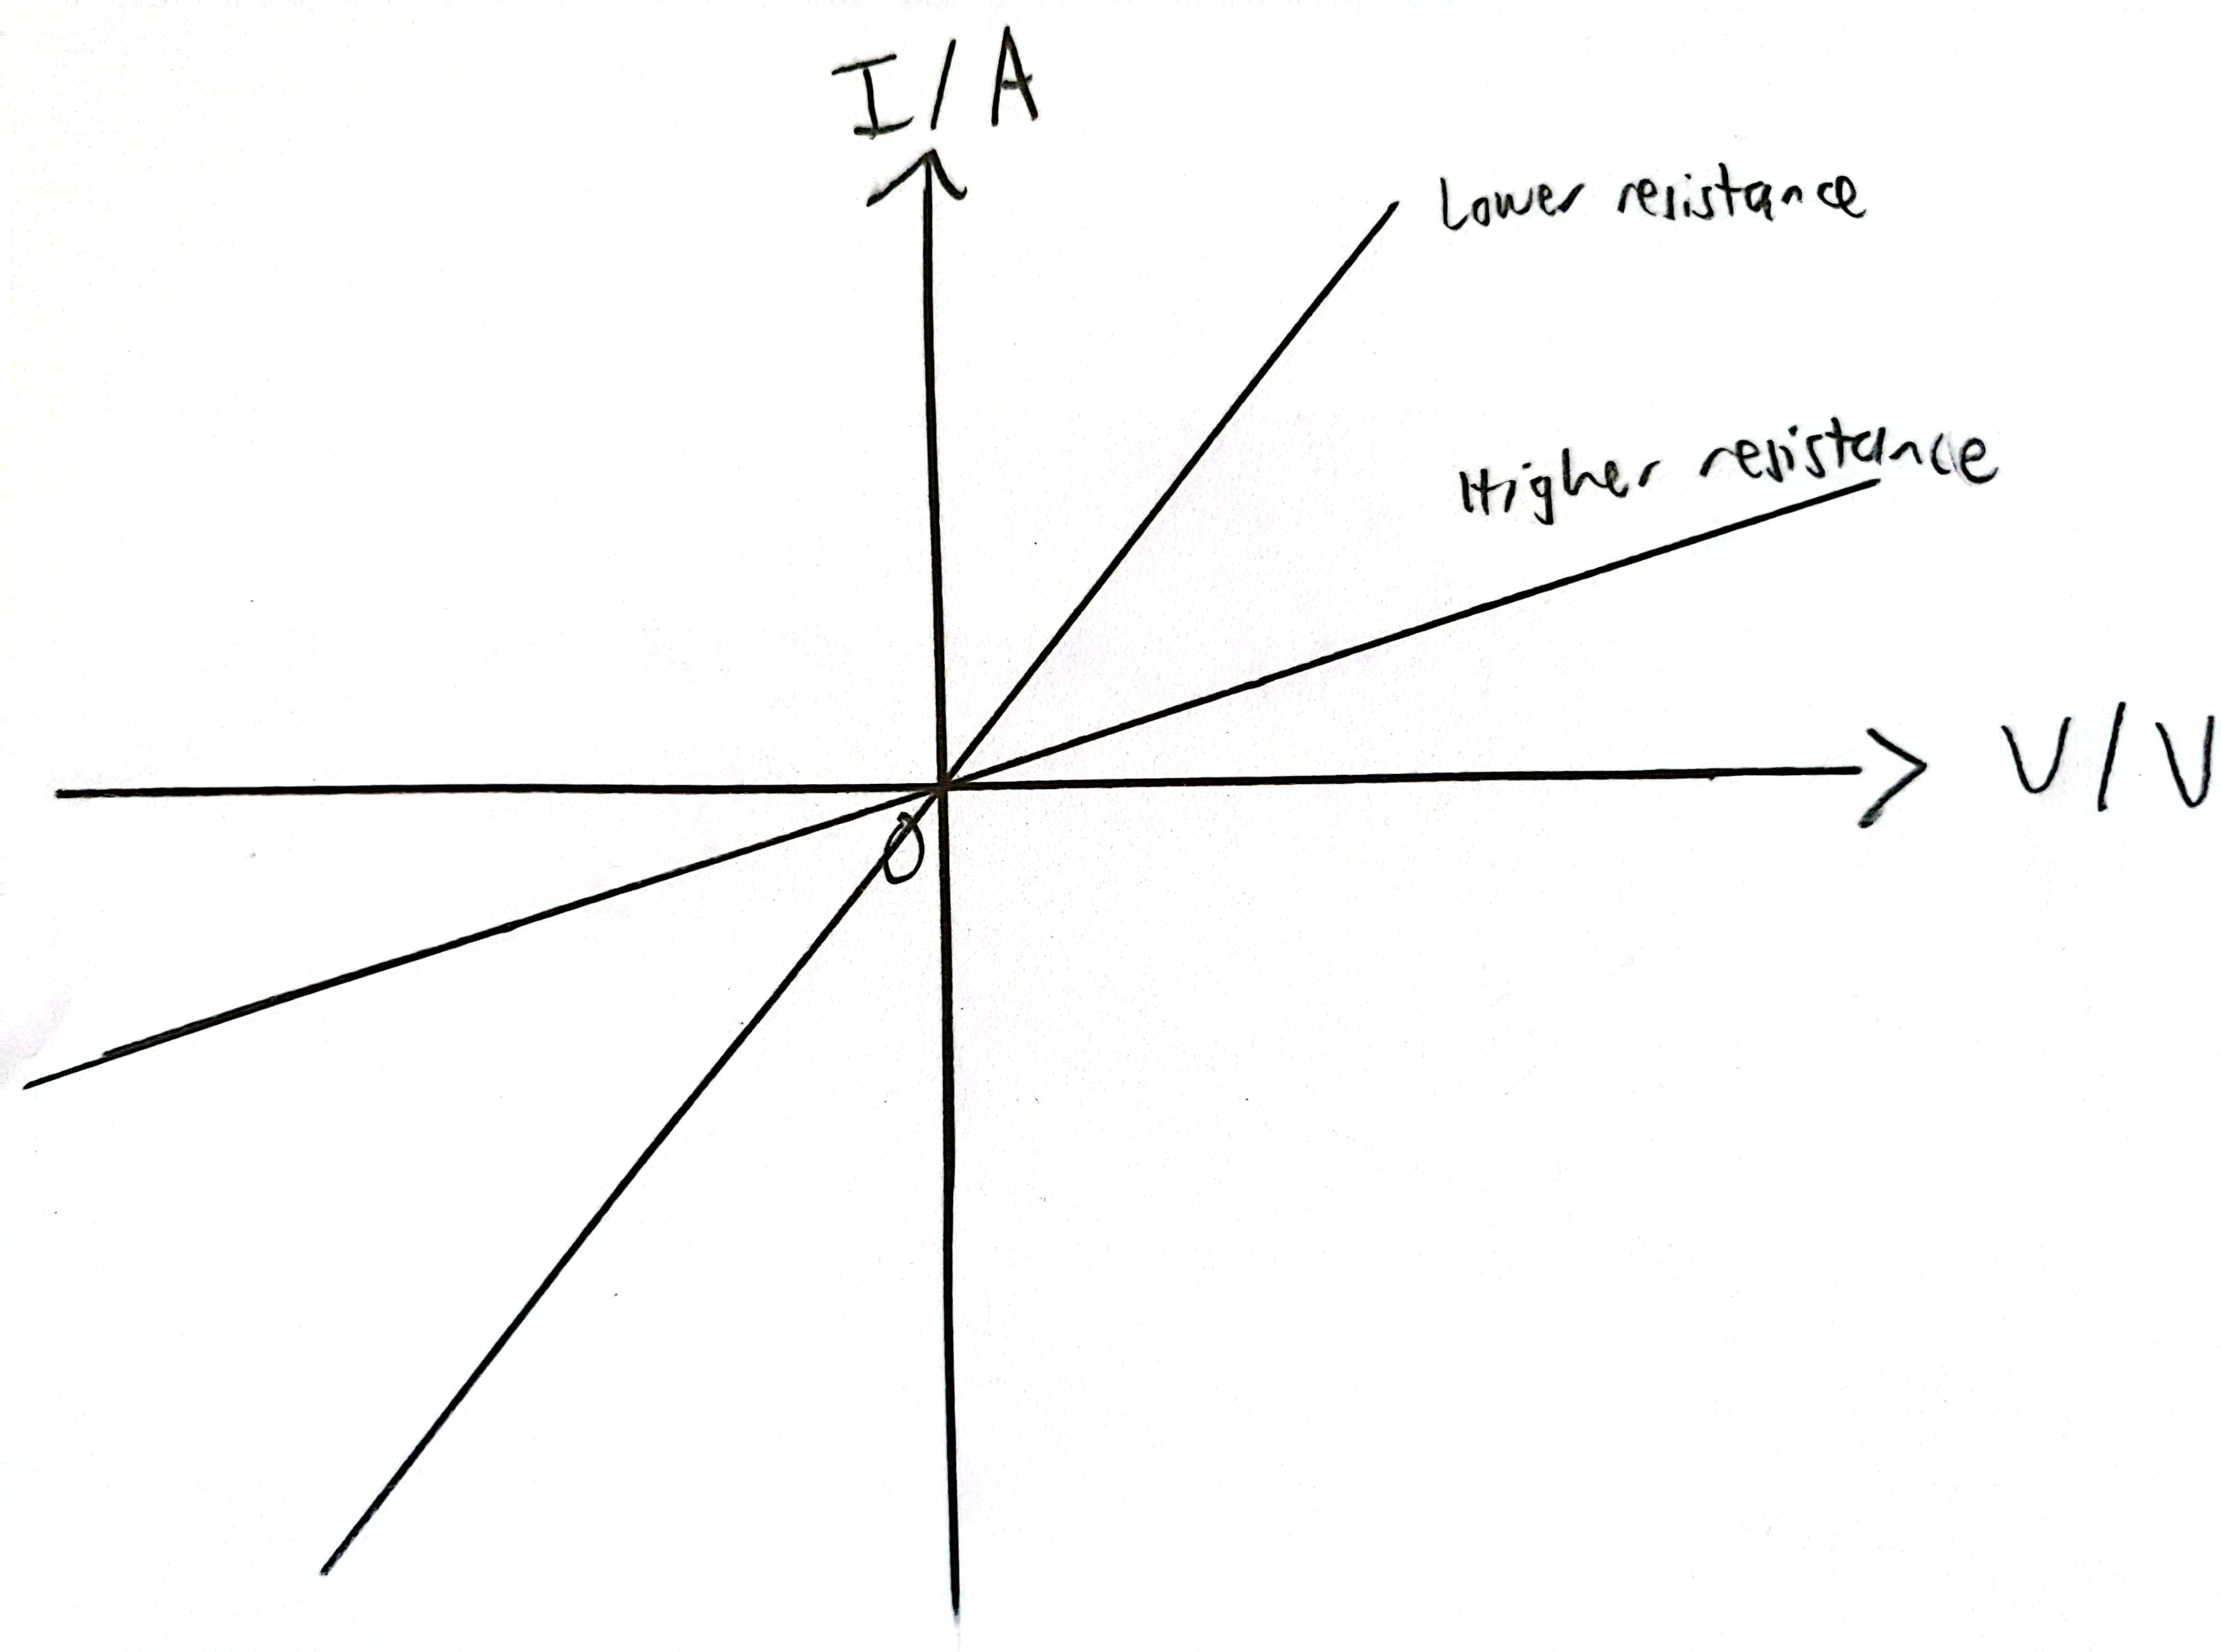
\includegraphics[width=\textwidth]{../images/MetallicConductor I-V.jpg}
        \end{minipage} &
        \begin{minipage}{0.3\textwidth}
            \begin{itemize}
                \item At \emph{constant temperature}, the \emph{number of free electrons} and the \emph{rate of atomic vibration} is constant.
                \item A resistor at a different constant temperature will have a difference resistance, and hence, \(V/I\) ratio. 
            \end{itemize}
        \end{minipage}\\
        \hline
        \begin{minipage}{0.25\textwidth}
            Semiconductor Diode\\[5mm]
            \begin{center}
                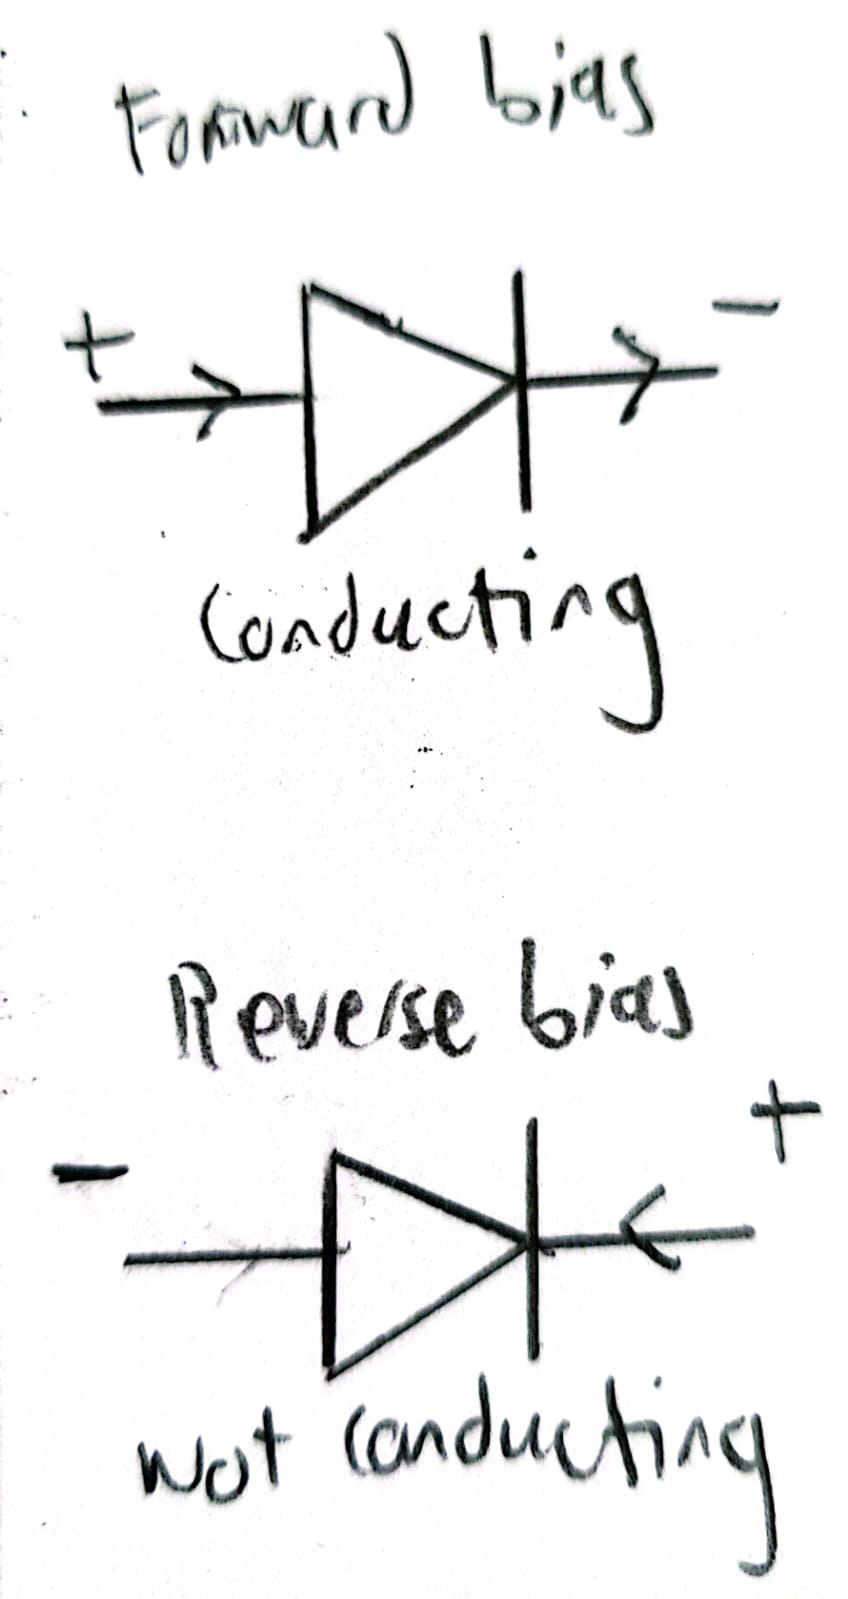
\includegraphics[scale=0.08]{../images/ForwardReverseBias.jpg}
            \end{center}
        \end{minipage} &
        \begin{minipage}{0.3\textwidth}
            \begin{itemize}
                    \item Forward-biased: \emph{Resistance decreases} when \emph{p.d. increases}. In fact, if the forward-biased p.d. goes past its \emph{threshold voltage}, \emph{resistance} becomes very low.
                    \item Reverse-biased: \emph{Very high resistance}. But, there will be a \emph{small leakage current}.
                    \item If the reverse-biased p.d. is so high that it exceeds the \emph{breakdown voltage}, the diode will \emph{break down} and \emph{conduct electricity}.
            \end{itemize} 
            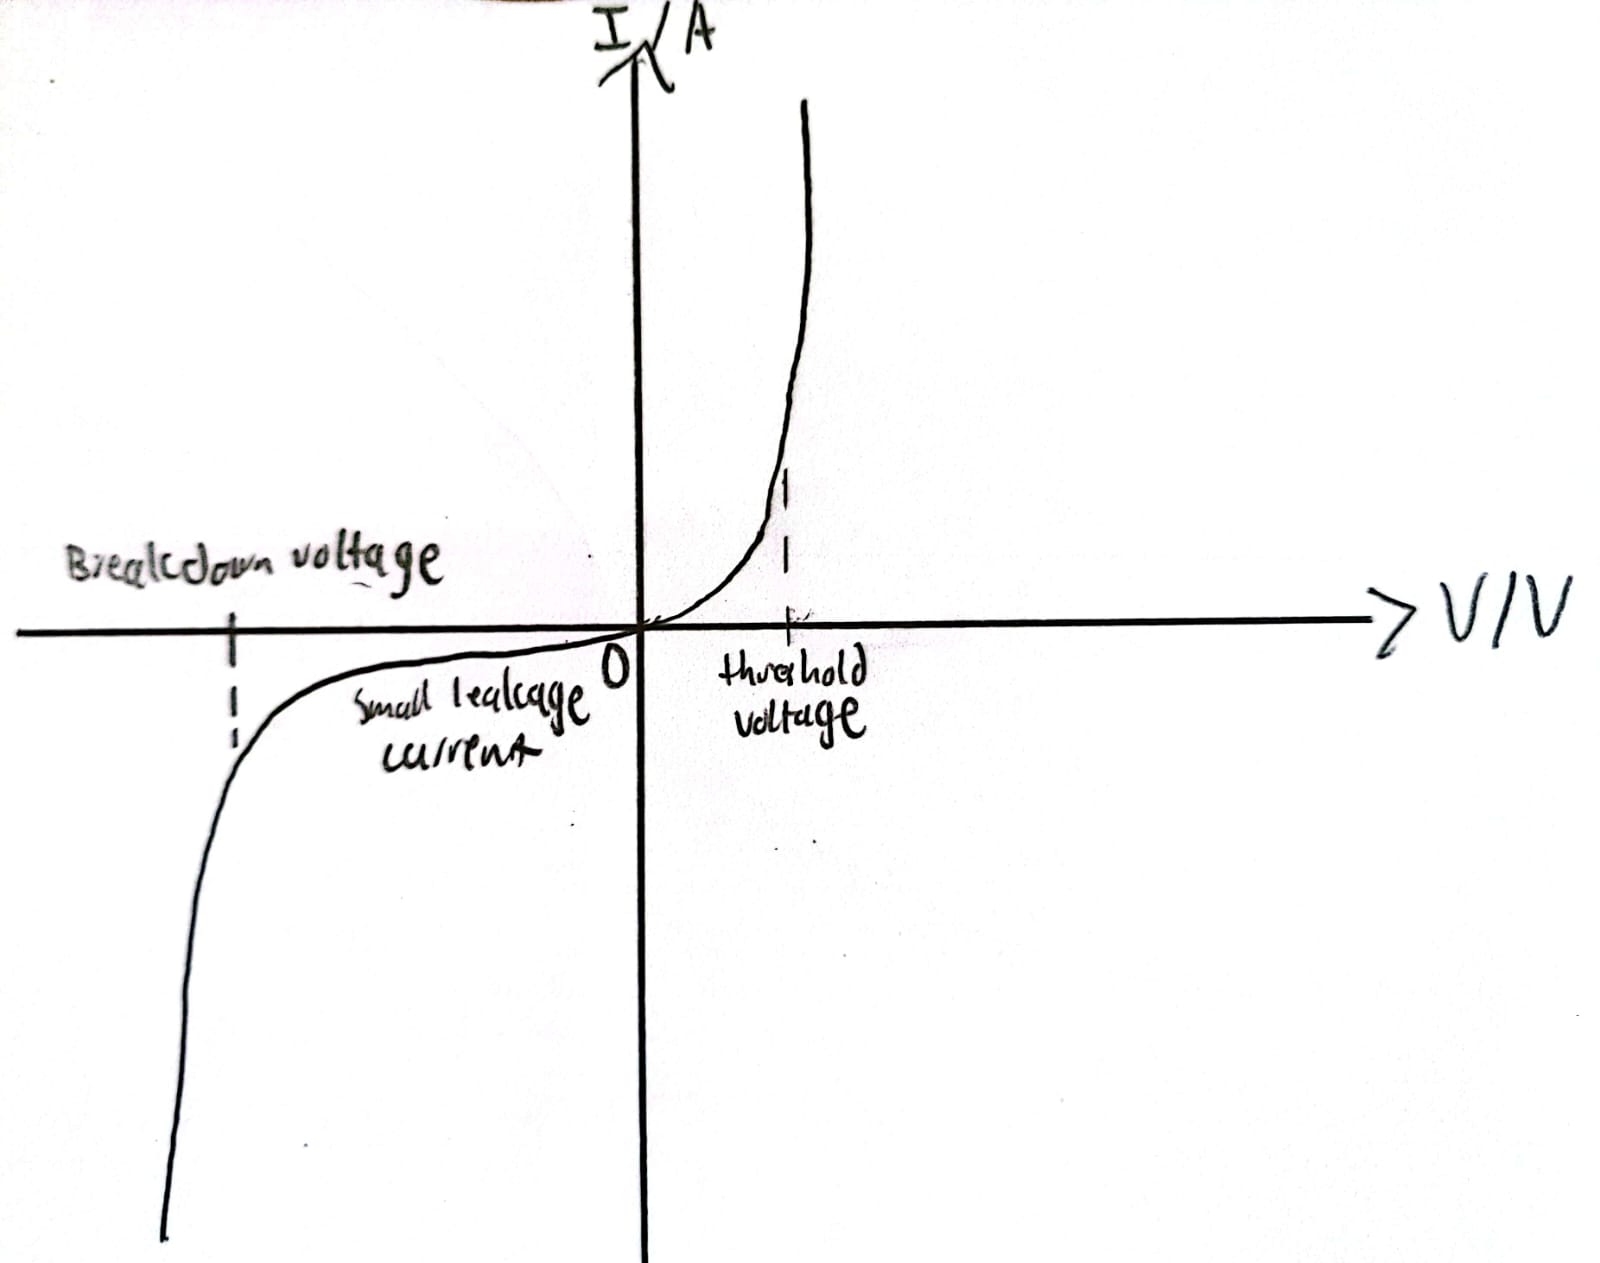
\includegraphics[width=\textwidth]{../images/Diode I-V characteristics.jpg}
        \end{minipage} &
        \begin{minipage}{0.3\textwidth}
            \begin{itemize}
                \item When connected in \emph{forward bias}, the circuit's \emph{electric field set up} allows for available \emph{charge carriers to flow} through, allowing it to conduct with \emph{low resistance}.
                \item When connected in \emph{reverse bias}, the circuit's electric field set up creates a \emph{widened `depletion region'} in the diode which \emph{impedes charge carriers} from flowing through the region, creating a \emph{large resistance}. 
            \end{itemize}
        \end{minipage}\\
        \hline
        \begin{minipage}{0.25\textwidth}
            Filament Lamp
        \end{minipage} &  
        \begin{minipage}{0.3\textwidth}
            \begin{itemize}
                \item When \emph{p.d. increases, current increases}, with \emph{decreasing \(I\)-\(V\) ratio}.
                \item The \emph{resistance} of a metallic conductor \emph{increases} with an increase in \emph{temperature}.
            \end{itemize} 
            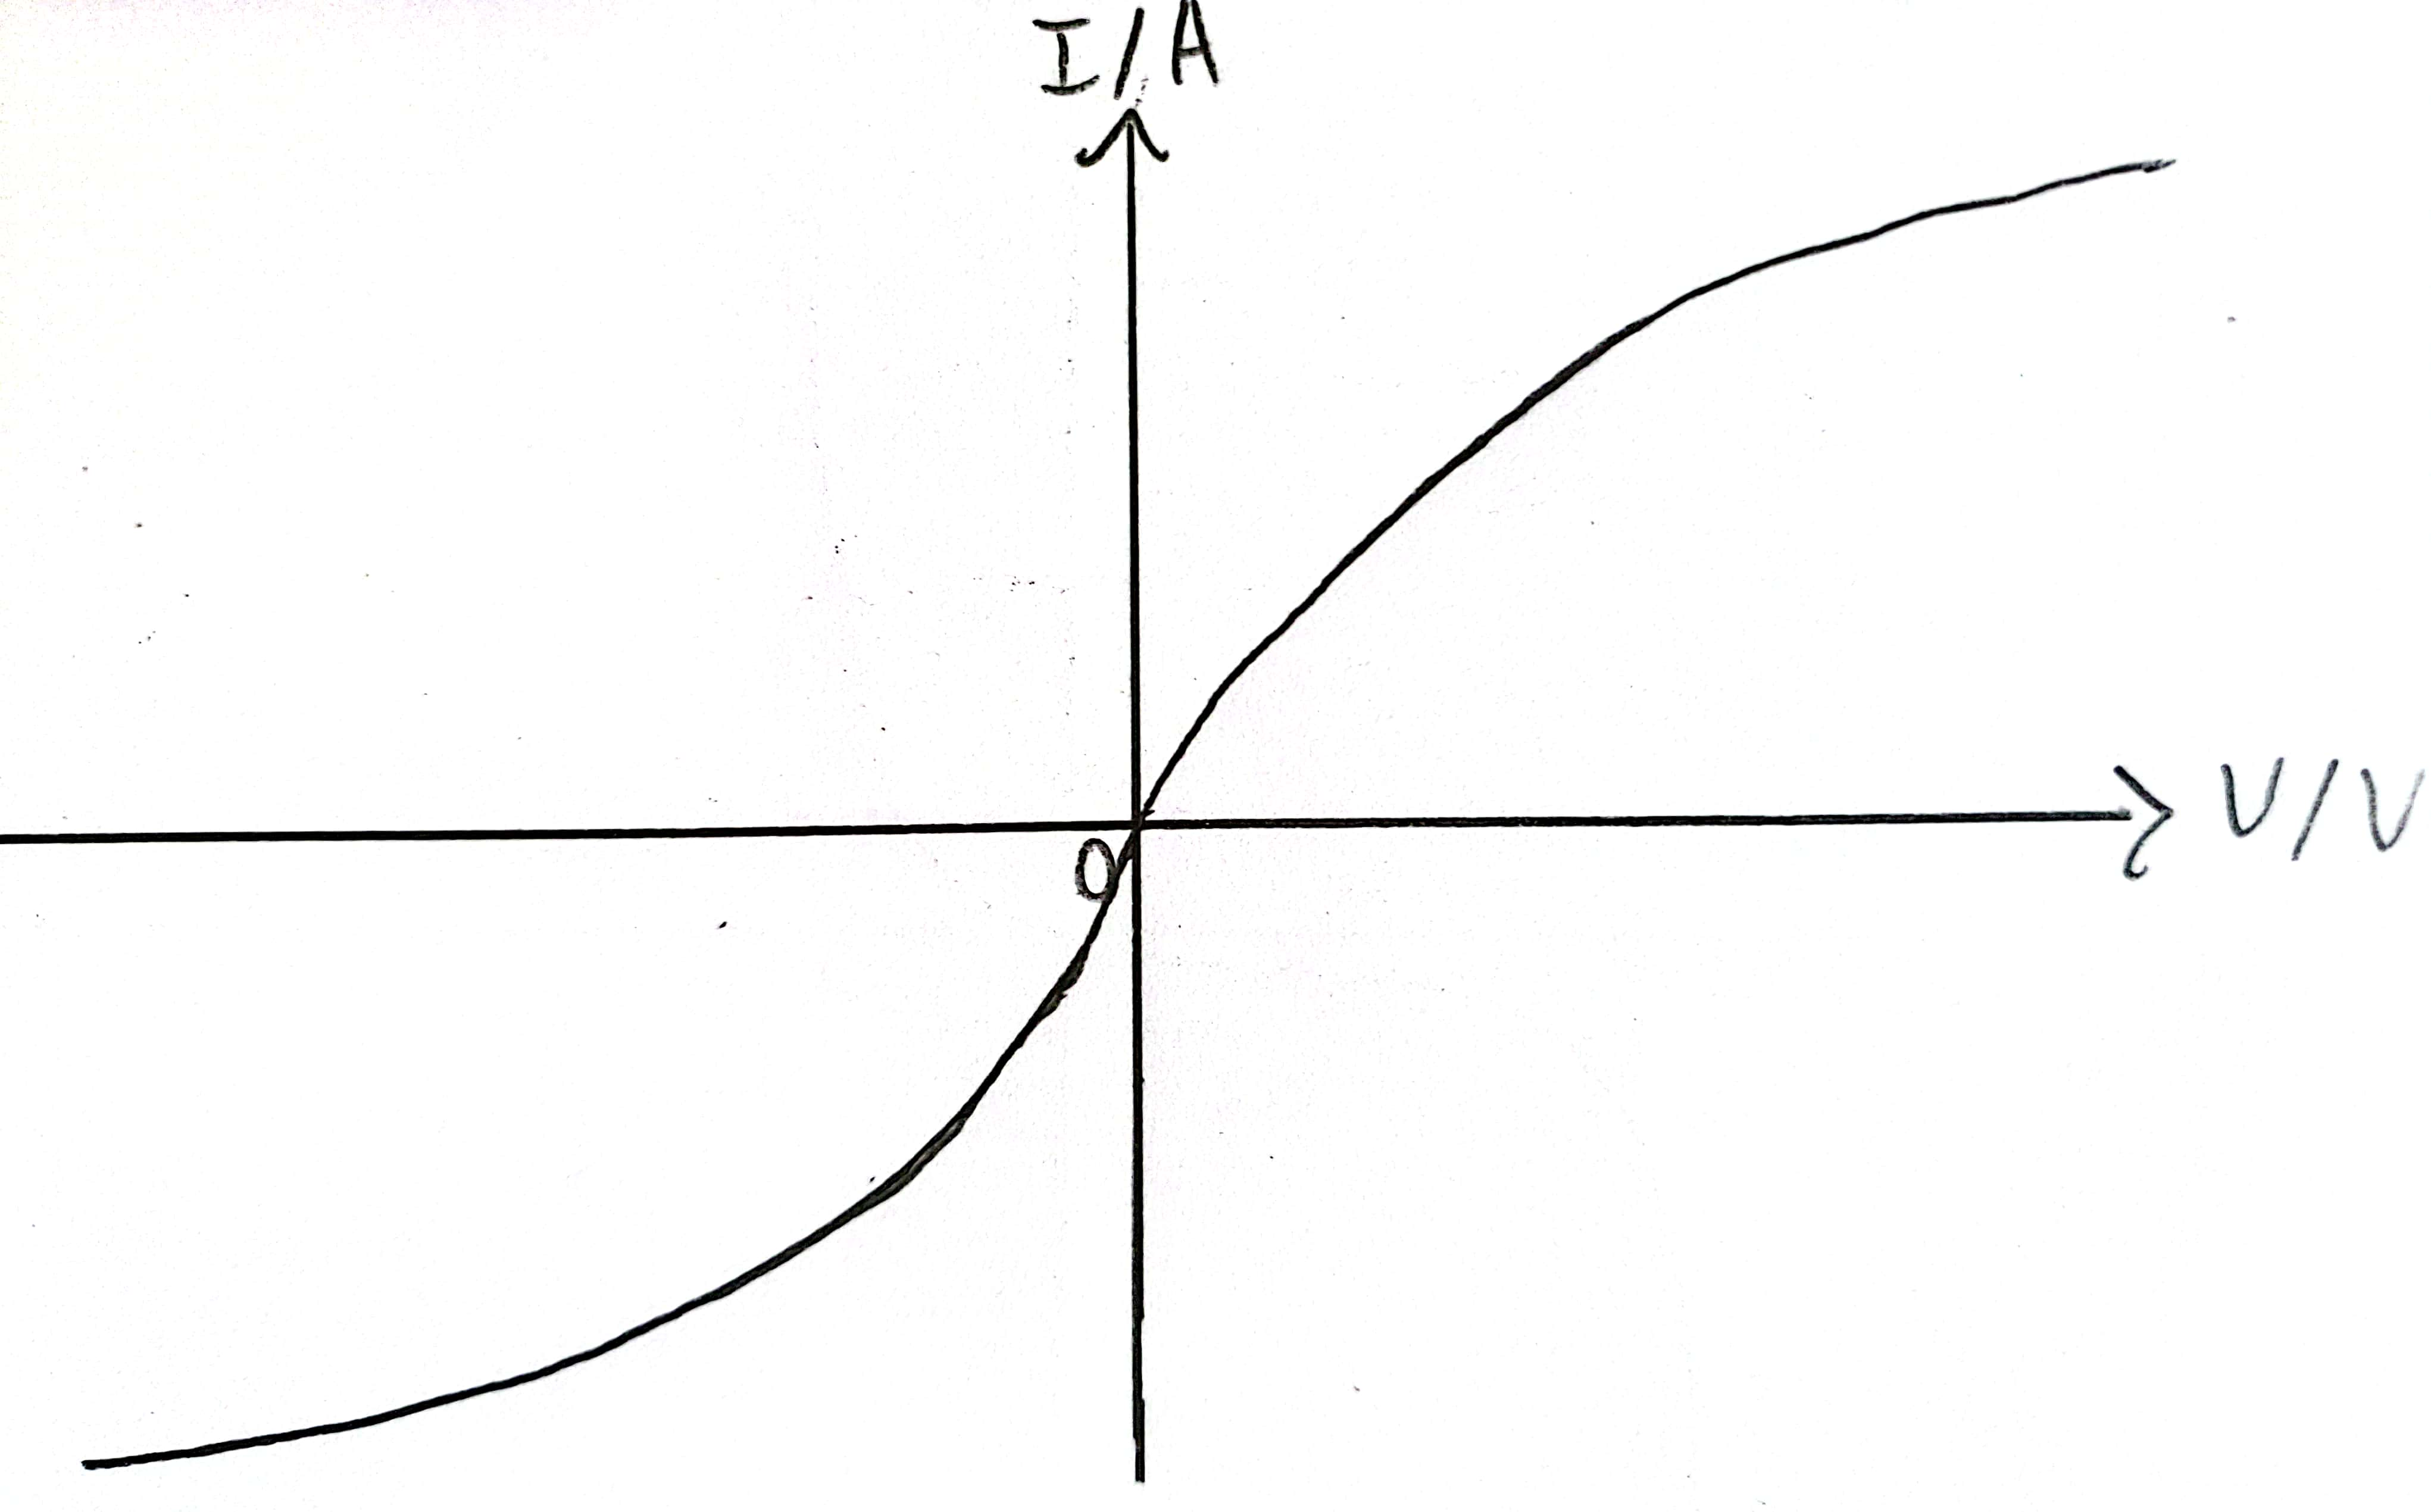
\includegraphics[width=\textwidth]{../images/Filament Lamp I-V Characteristics.jpg}\\[-1mm]
            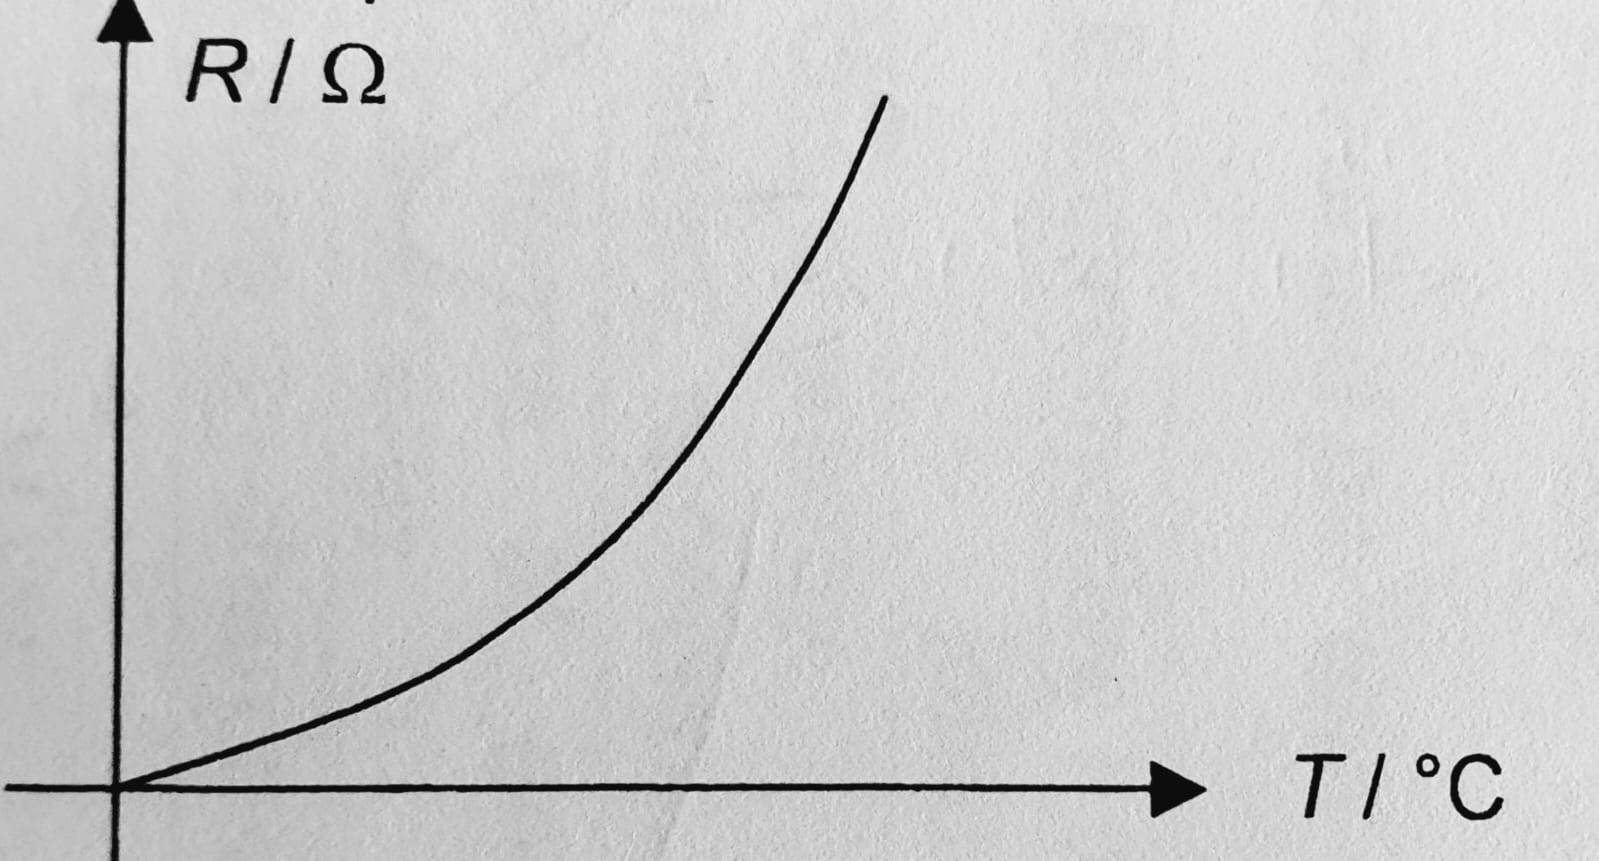
\includegraphics[width=\textwidth]{../images/Filament Lamp Resistance.jpg}
        \end{minipage} &
        \begin{minipage}{0.3\textwidth}
            \begin{itemize}
                \item As \emph{current increases, power dissipated increases} since \(P=I^2R\). Heat is generated so \emph{equilibrium temperature rises} --- as electrons drift through the metal, they collide with the metal lattice and transfers energy to it. 
                \item The \emph{lattice ions vibrate more vigorously}. This \emph{hinders the flow} of `charge carriers'. Therefore, \emph{resistance is increased}.
                \item Ohmic conductors hence do \emph{not} obey Ohm's Law at \emph{high} voltages/currents.
            \end{itemize}
        \end{minipage}\\
        \hline
        \begin{minipage}{0.25\textwidth}
            Negative Temperature Coefficient (NTC) Thermistor
        \end{minipage} &  
        \begin{minipage}{0.3\textwidth}
            \begin{itemize}
                \item When \emph{p.d. increases}, \emph{current} through the thermistor also \emph{increases}, with \emph{increasing \(I\)-\(V\) ratio}.
                \item The \emph{resistance} of a thermistor \emph{decreases} with an \emph{increase} in \emph{temperature} (This is the meaning of NTC).
            \end{itemize} 
            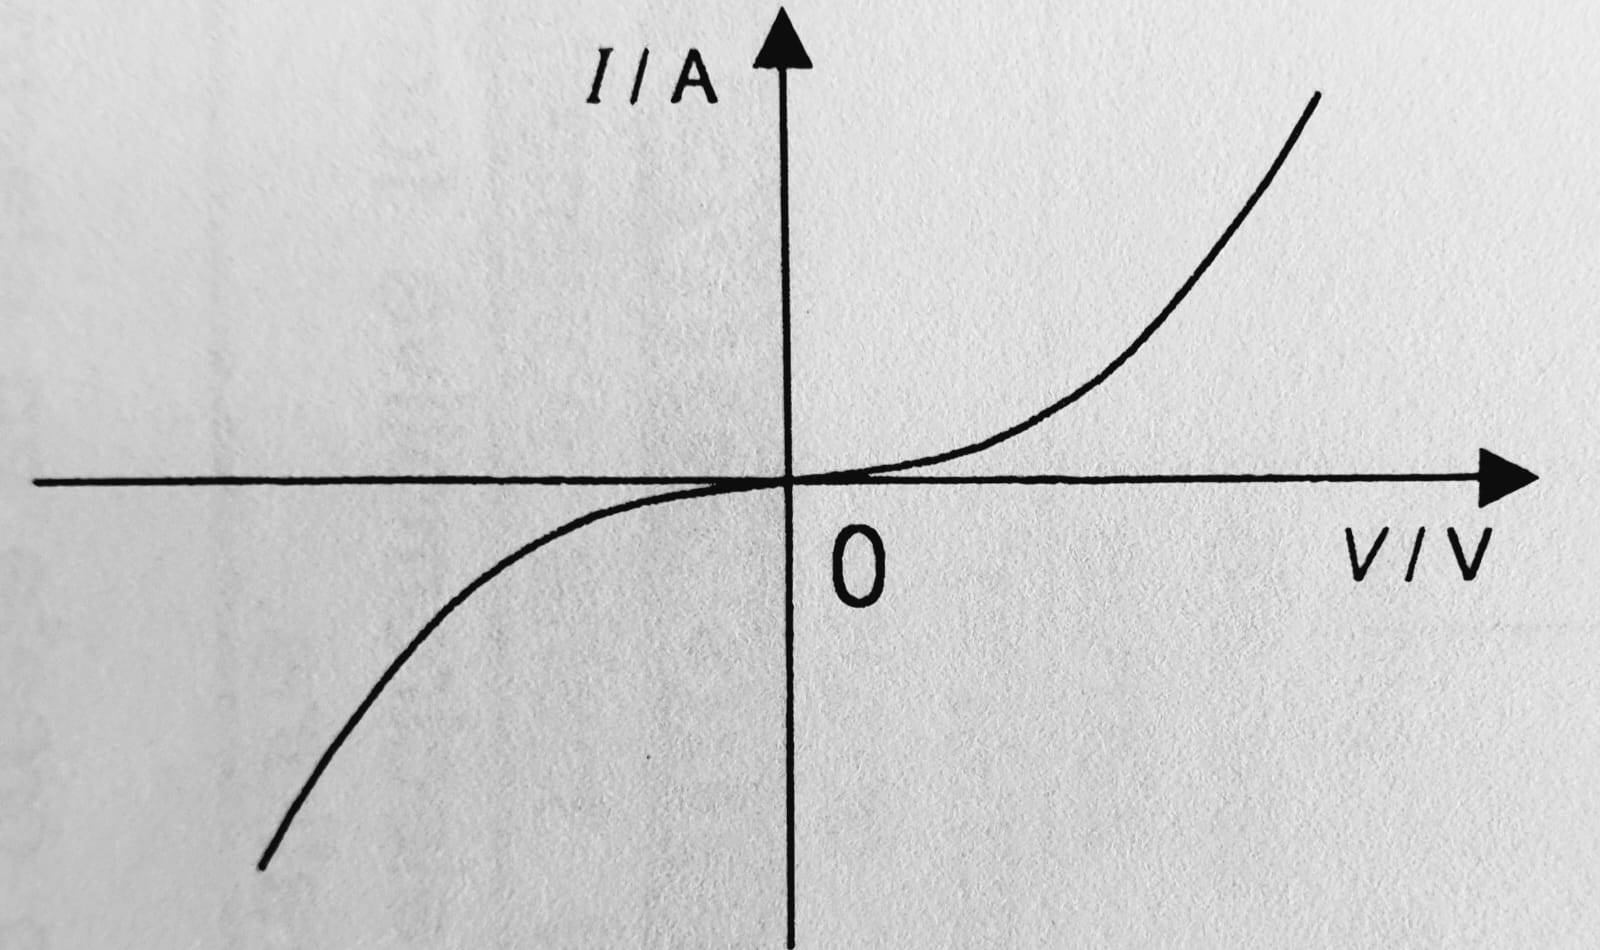
\includegraphics[width=\textwidth]{../images/NTC I-V.jpg}\\[-1mm]
            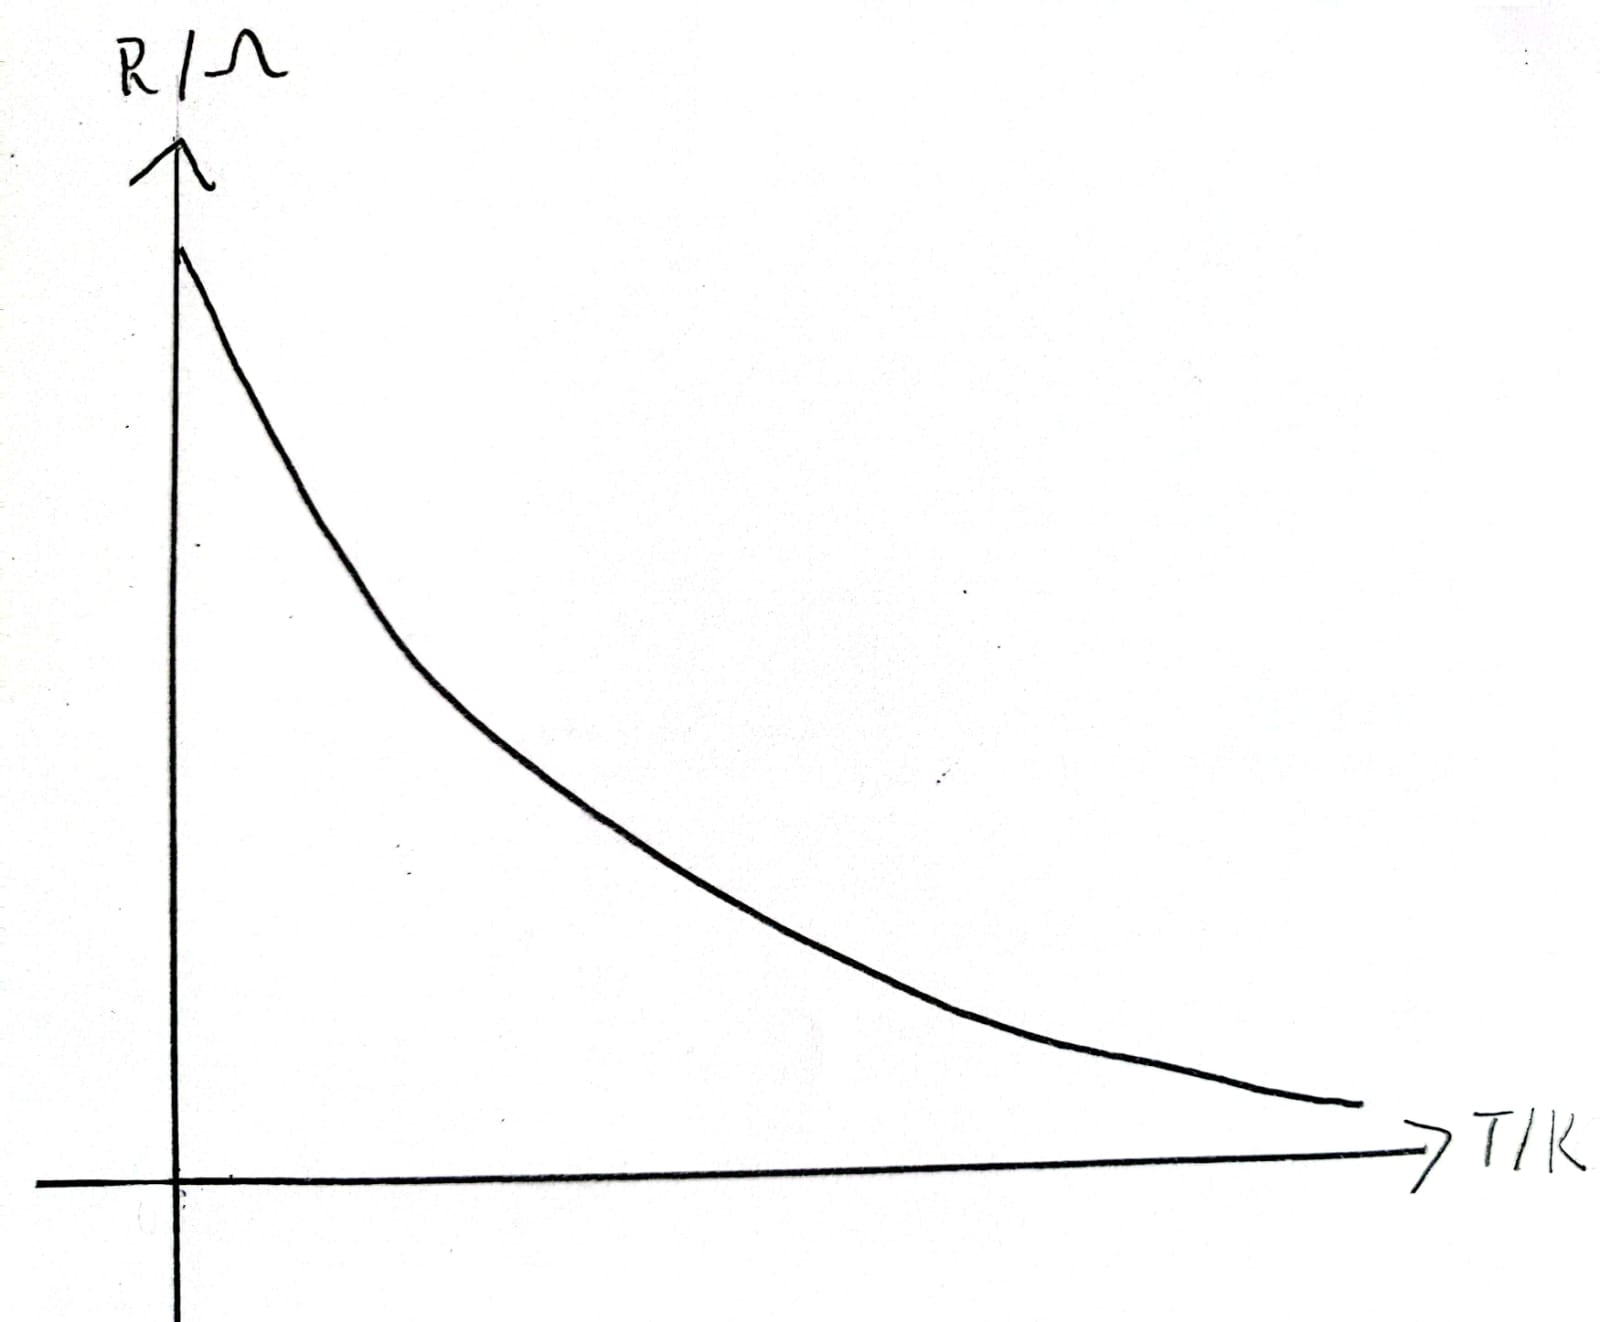
\includegraphics[width=\textwidth]{../images/NTC Resistance.jpg}
        \end{minipage} &
        \begin{minipage}{0.3\textwidth}
            \begin{itemize}
                \item  As \emph{current increases}, \emph{power dissipated increases}. \emph{More heat} is generated, leading to a \emph{rise} in \emph{equilibrium temperature}.
                \item Thus, the \emph{mean kinetic energy} of the electrons and lattice ions \emph{increases}. So,
            \end{itemize}
            \begin{enumerate}
                \item The \emph{bonded electrons break free} from bonds, increasing the \emph{number} of `mobile charge carriers'. Therefore, \emph{resistance decreases}.
                \item The \emph{lattice ions vibrate more vigorously}, \emph{hindering the flow} of `mobile charge carriers'. Thence, resistance increases.  
            \end{enumerate} 
            \begin{itemize}
                \item The first effect is much more significant than the second. So, there is a net \emph{decrease in resistance}.
            \end{itemize}
        \end{minipage}\\
        \hline
    \end{longtable}
    The images above come from \ref{RVHS}.
    \newpage
    \item The \emph{electromotive force} (e.m.f) of a \emph{source} is defined as the amount of \emph{energy converted} from \emph{non-electrical} forms of energy to \emph{electrical} energy \emph{per unit charge} as the \emph{charge passes through a complete circuit}.
    \item Internal resistance: the p.d. across a component is given by \(V=E-Ir\).
    \item Power dissipated \(P=IV\).
    \item Power delivered is \emph{maximum } when \(R=r\), such that 
    \[P_{\text{max}}=\frac{E^2}{4r}.\]
    \item Efficiency of the source
    \begin{itemize}
        \item \emph{Increases} when external load/\emph{resistance increases}.
        \item Is halved when \(R=r\).

        \emph{Note:} Maximum power \(\neq\) maximum efficiency.
    \end{itemize}
\end{itemize}

\chapter{Electric Fields}
\begin{itemize}
    \item \emph{Coulomb's Law} states that the \emph{magnitude} of the \emph{electric force} between two \emph{point charges} is directly proportional to the product of the charges, and inversely proportional to the square of their separation.
    \item The constant \(\varepsilon_0\) is the permittivity of \emph{free space} (\(\varepsilon_0\) is applicable only in air or a vacuum).
    \item Sign of \(F_E\):
    \begin{center}
        \begin{tabular}{|Sc|Sc|}
            \hline
            \(F_E\) & Direction\\
            \hline
            Positive & Repulsive\\
            \hline
            Negative & Attractive\\ 
            \hline
        \end{tabular}  
    \end{center}
    
  \item The sign of the electric force does \emph{not} represent the \emph{direction} of the electric force. It only informs us whether the force is attractive or repulsive. So, when calculating the \emph{resultant} electric force, we need to account for the direction ourselves. 
    \item Comparison between E-fields and G-fields: 
    \begin{center}
        \resizebox{0.942\textwidth}{!}{\begin{tabular}{|Sc|Sc|Sc|}
            \hline
            Sim/Diff & E-field & G-field\\
            \hline
            S & 
            \multicolumn{2}{Sc|}{\begin{minipage}{0.8\textwidth}
            For both Column's Law and Newton's Law of Gravitation, \(r\) is the \emph{center to center separation} of the objects.
            \end{minipage}}\\
            \hline
            S & 
            \multicolumn{2}{Sc|}{\begin{minipage}{0.8\textwidth}
            By Newton's Third Law, the \emph{forces} that masses and charges exert on each other is \emph{equal in magnitude} and \emph{opposite in direction}.
            \end{minipage}}\\
            \hline
            D & 
            \begin{minipage}{0.4\textwidth}
                Electric Forces can be \emph{attractive or repulsive}.
            \end{minipage} &
            \begin{minipage}{0.4\textwidth}
                Gravitational forces are \emph{always attractive}.
            \end{minipage}\\
            \hline 
    \end{tabular}}
    \end{center}
    \item An \emph{electric field} is a \emph{region in space} where a \emph{charge experiences an electric force}.
    \item How to draw electric field lines: 
    \begin{itemize}
        \item \emph{Lines cannot intersect} one another.
        \item Lines must \emph{begin from positive charges} and \emph{end on negative charges}.
        \item Arrows show the \emph{direction of force} exerted on a positive test charge.
        \item The \emph{greater} the electric field strength, the \emph{closer} together field lines are drawn.
        \item Lines leave/end on \emph{conducting surfaces} at \emph{right angles}
    \end{itemize}
    % POINT CHARGE +1
    \resizebox{0.942\textwidth}{!}{\begin{tikzpicture}
    \foreach \i [evaluate={\angle=(\i-1)*360/\NE;}] in {1,...,\NE}{
      \draw[EFieldLineArrow={0.6}] (0,0) -- (\angle:\R);
    }
    \draw[charge+] (0,0) circle (7pt) node[black,scale=0.8] {$+q$};
  \end{tikzpicture}
  % POINT CHARGE -1
  \begin{tikzpicture}
    \foreach \i [evaluate={\angle=(\i-1)*360/\NE;}] in {1,...,\NE}{
      \draw[EFieldLineArrow={0.5}] (\angle:\R) -- (0:0);
    }
    \draw[charge-] (0,0) circle (7pt) node[black,scale=0.8] {$-q$};
  \end{tikzpicture}
  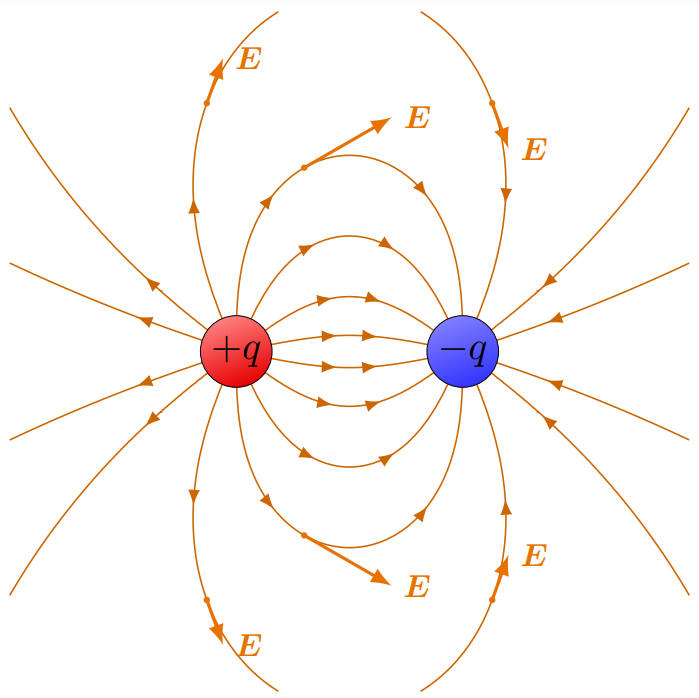
\includegraphics[width=0.25\textwidth]{../images/2 charges.png}
  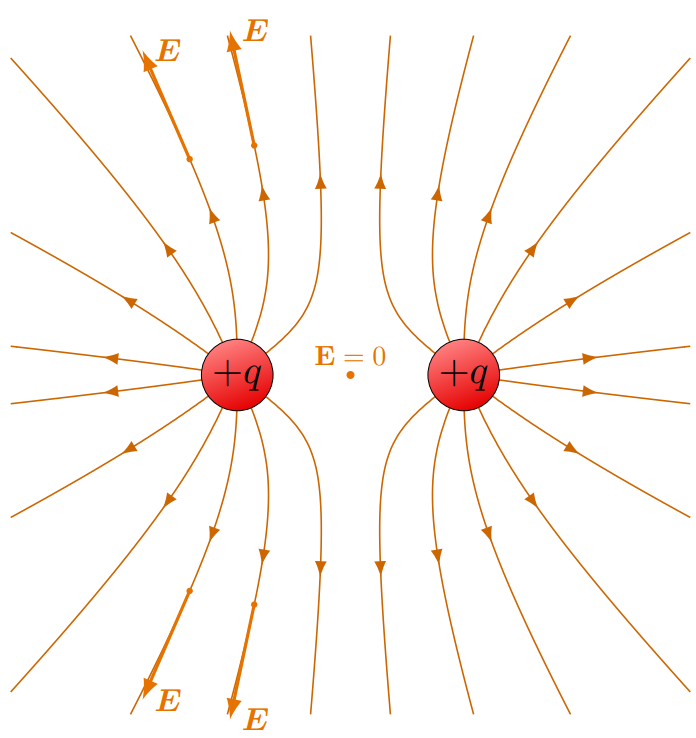
\includegraphics[width=0.25\textwidth]{../images/2repellingcharges.png}}
  \captionsetup{type=figure}
  \caption[figure]{\ref{Electric field lines of a point charge}, \ref{Electric field lines of two charges} Electric field lines of point charges and two interacting charges.}
  \begin{center}
    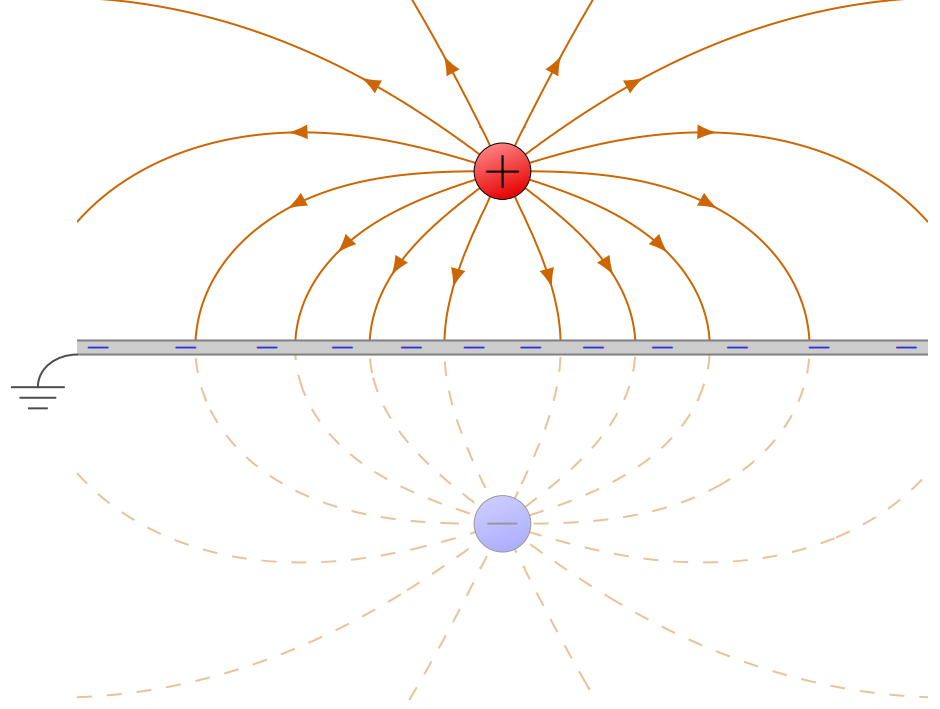
\includegraphics[width=0.5\textwidth]{../images/E-fieldPlate.png}
    \captionsetup{type=figure}
    \caption[figure]{\ref{Interaction of a point charge with a charged plate} Interaction of a point charge with a charged plate.}
  \end{center}
  \item The \emph{electric field strength} at a point is defined as the \emph{electric force} per \emph{unit positive charge} acting on a small stationary test charge placed at that point.
  \begin{center}
    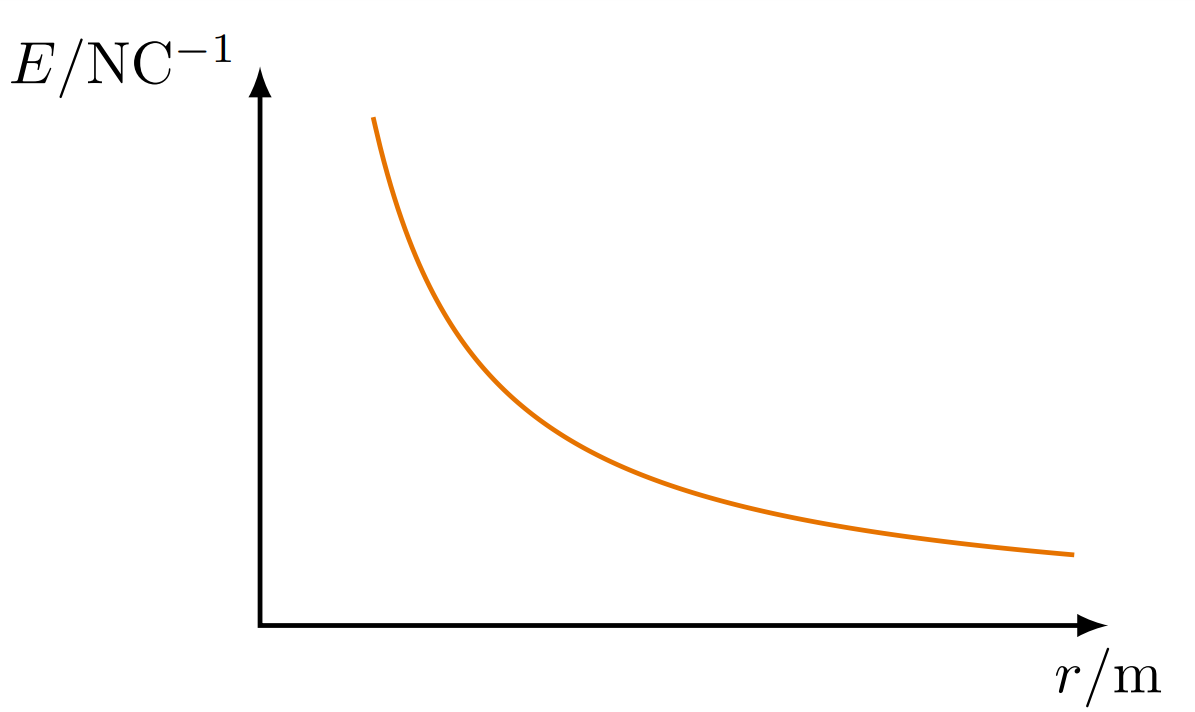
\includegraphics[width=0.5\textwidth]{../images/ElectricFieldStrengthPlot.png}
    \captionsetup{type=figure}
    \caption[figure]{\ref{Electric field plots} Electric field strength of a positive point charge}
  \end{center}
  \item Charge distribution on a conducting sphere: 
  \begin{itemize}
    \item Excess charges are forced to the surface of the conductor until the electric field inside the conductor is zero. 
    \item \emph{Outside} the conductor, the electric field is the \emph{same} as that of an isolated point charge equal to the excess charge. 
  \end{itemize}
  \item Properties of conductors in \emph{electrostatic equilibrium}:
  \begin{itemize}
    \item The \emph{electric field is zero inside} a conductor (regardless of shape).
    \item So, the \emph{entire conductor} is at the \emph{same potential}.
    \item Just outside the conductor, the e-field lines are \emph{perpendicular to its surface}, starting and ending on charges on the surface.
    \item \emph{Excess charges} resides exclusively on \emph{the surfaces} of a conductor.
  \end{itemize}
  \item Electric field strength between two charged parallel plates is uniform everywhere between the plates, except at both ends of the plates. 
  \item Also, \emph{charges} between the plates experience \emph{uniform acceleration}.
  \begin{center}
    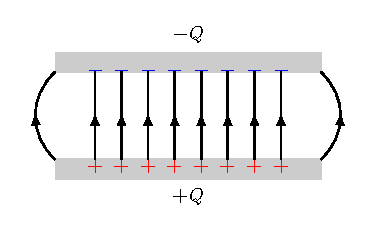
\includegraphics[scale=1]{../images/ParallelPlates/testing.pdf}
    \captionsetup{type=figure}
    \caption[figure]{\ref{Electric field lines between parallel plates} Electric field lines between parallel plates.}
  \end{center}
  \item Magnitude of electric field strength between the plates:
  \[E=\frac{dV}{dr}=\frac{\Delta V}{d}.\]
  \item The \emph{electric potential energy} of a point charge in an electric field is defined as the \emph{work done by an external agent} in bringing the point charge from infinity to that point (without any net change in kinetic energy). 
  \item The \emph{electric potential} at a point in an electric field is defined as the \emph{work done} per unit \emph{positive} charge, by an external agent, in bringing a \emph{small} test charge from infinity to that point (without any net change in kinetic energy). 
  \item Let \(U\) be the electric potential energy, and \(V\) the electric potential. Then,
  \[U=qV \qquad\text{and}\qquad \Delta U=q\Delta V.\]
  \item ~
  \begin{center}
    \begin{tikzcd}[row sep=large, column sep=large]
        U=\frac{Qq}{4\pi\varepsilon_0r} \arrow{r}{-\frac{\text{d}}{\text{d}r}} \arrow[swap]{d}{\frac{1}{q}} & F_E=\frac{Q_1Q_2}{4\pi\varepsilon_0r^2} \arrow[swap]{d}{\frac{1}{q}} \\
        V=\frac{Q}{4\pi\varepsilon_0r} \arrow{r}{-\frac{\text{d}}{\text{d}r}} & E=\frac{Q}{4\pi\varepsilon_0r^2}\\
    \end{tikzcd}
  \end{center}
  \item The \emph{electric potential} at a point \(X\) due to a \emph{system} of point charges \(q_i\) is the algebraic sum of the electric potential \(V_i\) due to each individual charge \(q_i\) which is distance \(r_i\) away from \(X\). That is, 
  \[V=\sum_{i}{V_i}=\sum_{i}^{}{\frac{q_i}{4\pi\varepsilon_0r_i}}.\]
  \item The \emph{potential energy} of a \emph{system} of charges \(q_i\) is the work done to assemble it. This is the sum of energies \(U_{ij}\) needed to bring each charge \(q_i\) to the charges \(q_j\) (for \(i>j\)) already present. In other words letting \(r_{ij}\) be the distance of \(q_i\) from \(q_j\), we have 
  \[U=\sum_{i>j}{U_{ij}}=\sum_{i>j}^{}{\frac{q_iq_j}{4\pi\varepsilon_0r_{ij}}}.\] 
\end{itemize}
\begin{center}
    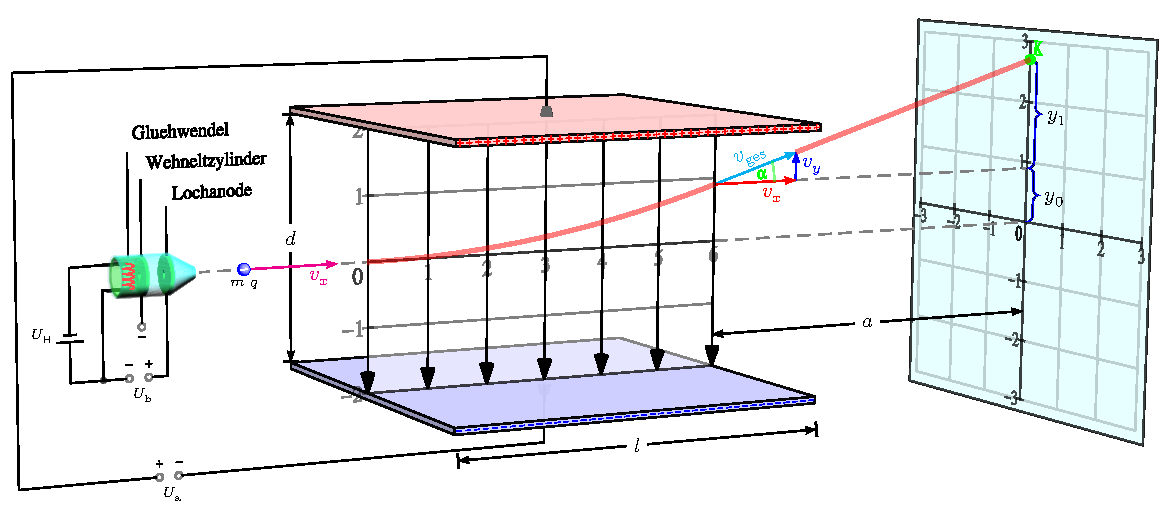
\includegraphics[width=\textwidth]{../images/Electron-Deflection/Bahn-Kondensator (1).pdf}
    \captionsetup{type=figure}
    \caption[figure]{\ref{Electron deflection} Deflection of an electron.}
\end{center}

\chapter{D.C. Circuits}
\begin{center}
    \begin{tabular}{|Sc|Sc|Sc|}
        \hline
        Property & Series & Parallel\\
        \hline
        Current & \(I_1=I_2=\cdots=I_n\) & \(I_i=\dfrac{E}{R_i}\)\\
        \hline
        Resistance & \(R_{\text{effective}}=R_1+R_2+\cdots+R_n\) & \(\dfrac{1}{R_{\text{effective}}}=\dfrac{1}{R_1}+\dfrac{1}{R_2}+\cdots+\dfrac{1}{R_n}\)\\
        \hline
        Voltage & \(V_i=\dfrac{R_i}{R_T}\cdot E\) & \(E=V_1=V_2=\cdots=V_n\).\\
        \hline
    \end{tabular}
\end{center}
\begin{itemize}
    \item For \(n\) identical resistors in parallel, which are each of resistance \(R\), we have \(R_{\text{effective}}=R/n\). Furthermore, the effective resistance is at most the resistance of the smallest resistor, i.e. \(R_{\text{effective}}\leq R_i\) for each \(i\). In fact, the inequality is strict when the number of resistors in parallel \(n\geq 2\).
    \item To resolve tricky systems of resistors, use the fact that electric potential is constant along a wire.
    \begin{center}
        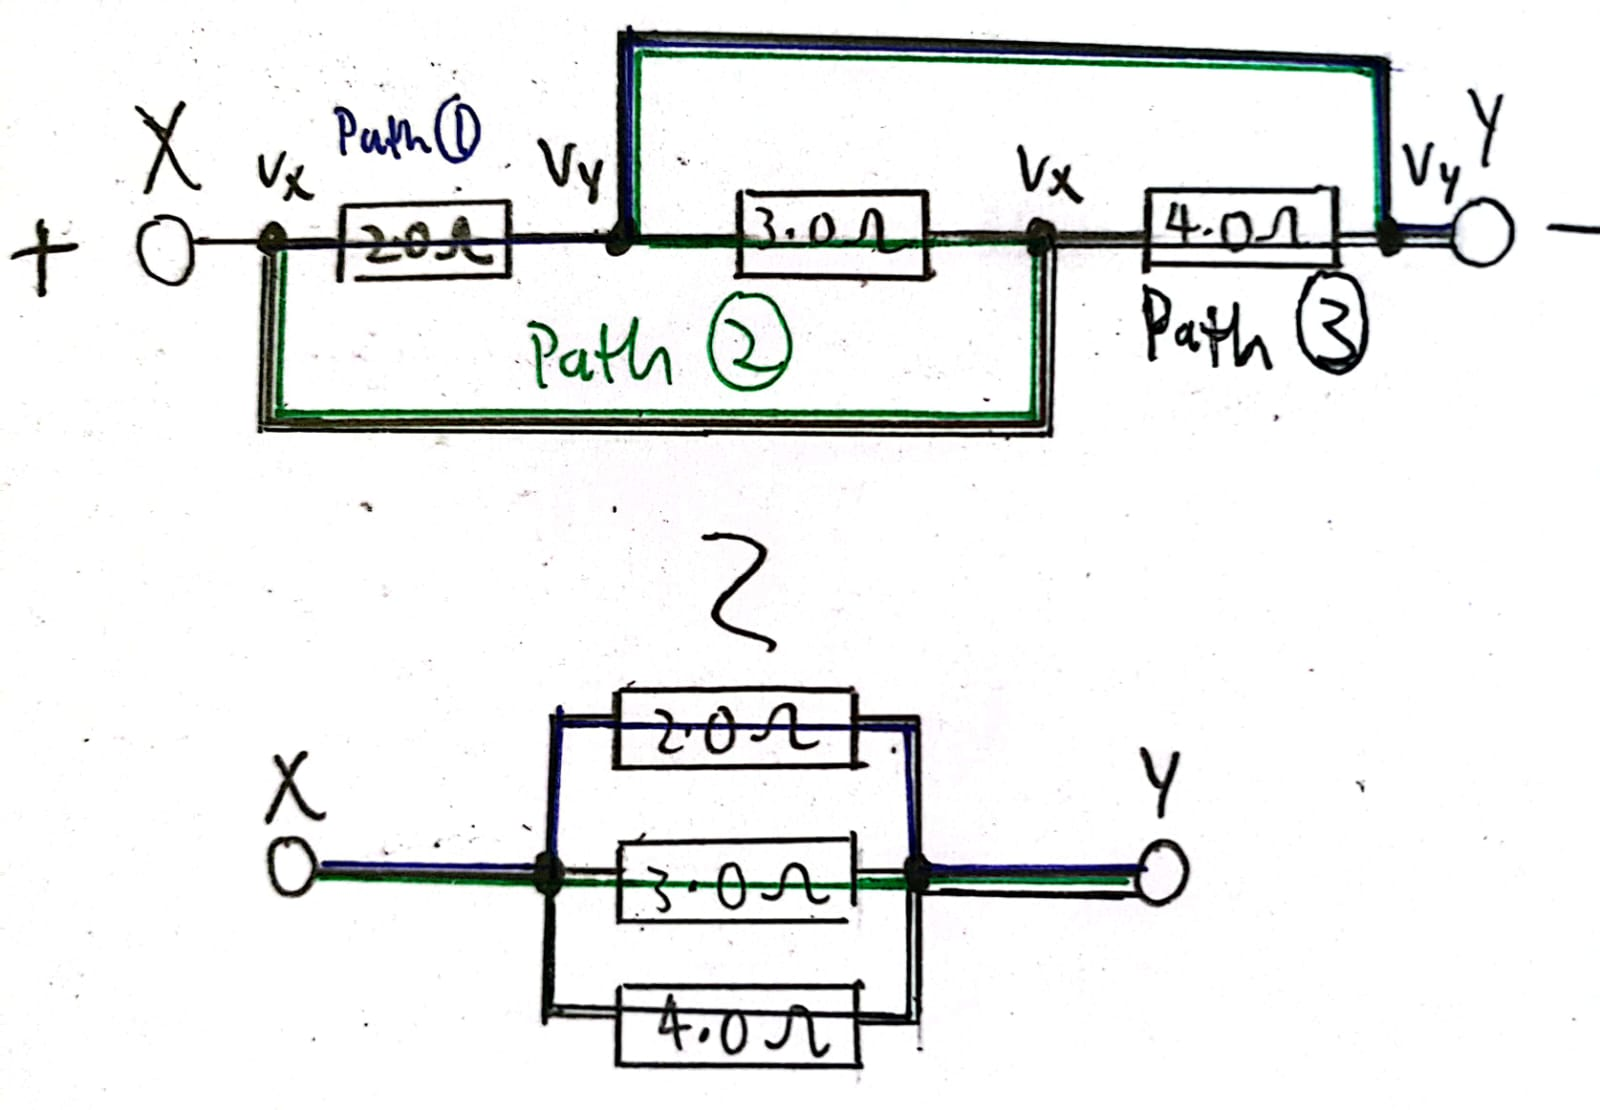
\includegraphics[width=0.93\columnwidth]{../images/DC-Circuits-Resistors.jpg}
        \captionsetup{type=figure}
        \caption[figure]{\ref{RVHS} Some tricky ciruits.}
    \end{center}
    \item Potentiometer:
    \begin{itemize}
        \item E.m.f. of driver cell is more than that of the unknown cell, \(E\).
        \item The direction of charge flow for the primary and secondary circuits are opposite. i.e. the positive/negative terminals should `point' towards each other.
        \item The potential difference \(V\) across length \(L\) of a resistance wire is directly proportional to \(L\).
        \item Consider the following circuit. When the galvanometer reads zero, the e.m.f. of the unknown cell is \(E_{AJ}\), where 
        \[\frac{E_{\text{AJ}}}{E}=\frac{L_{\text{AJ}}}{L_{\text{AB}}}=\frac{R_{\text{AJ}}}{R_{\text{AB}}}.\]
        \begin{center}
            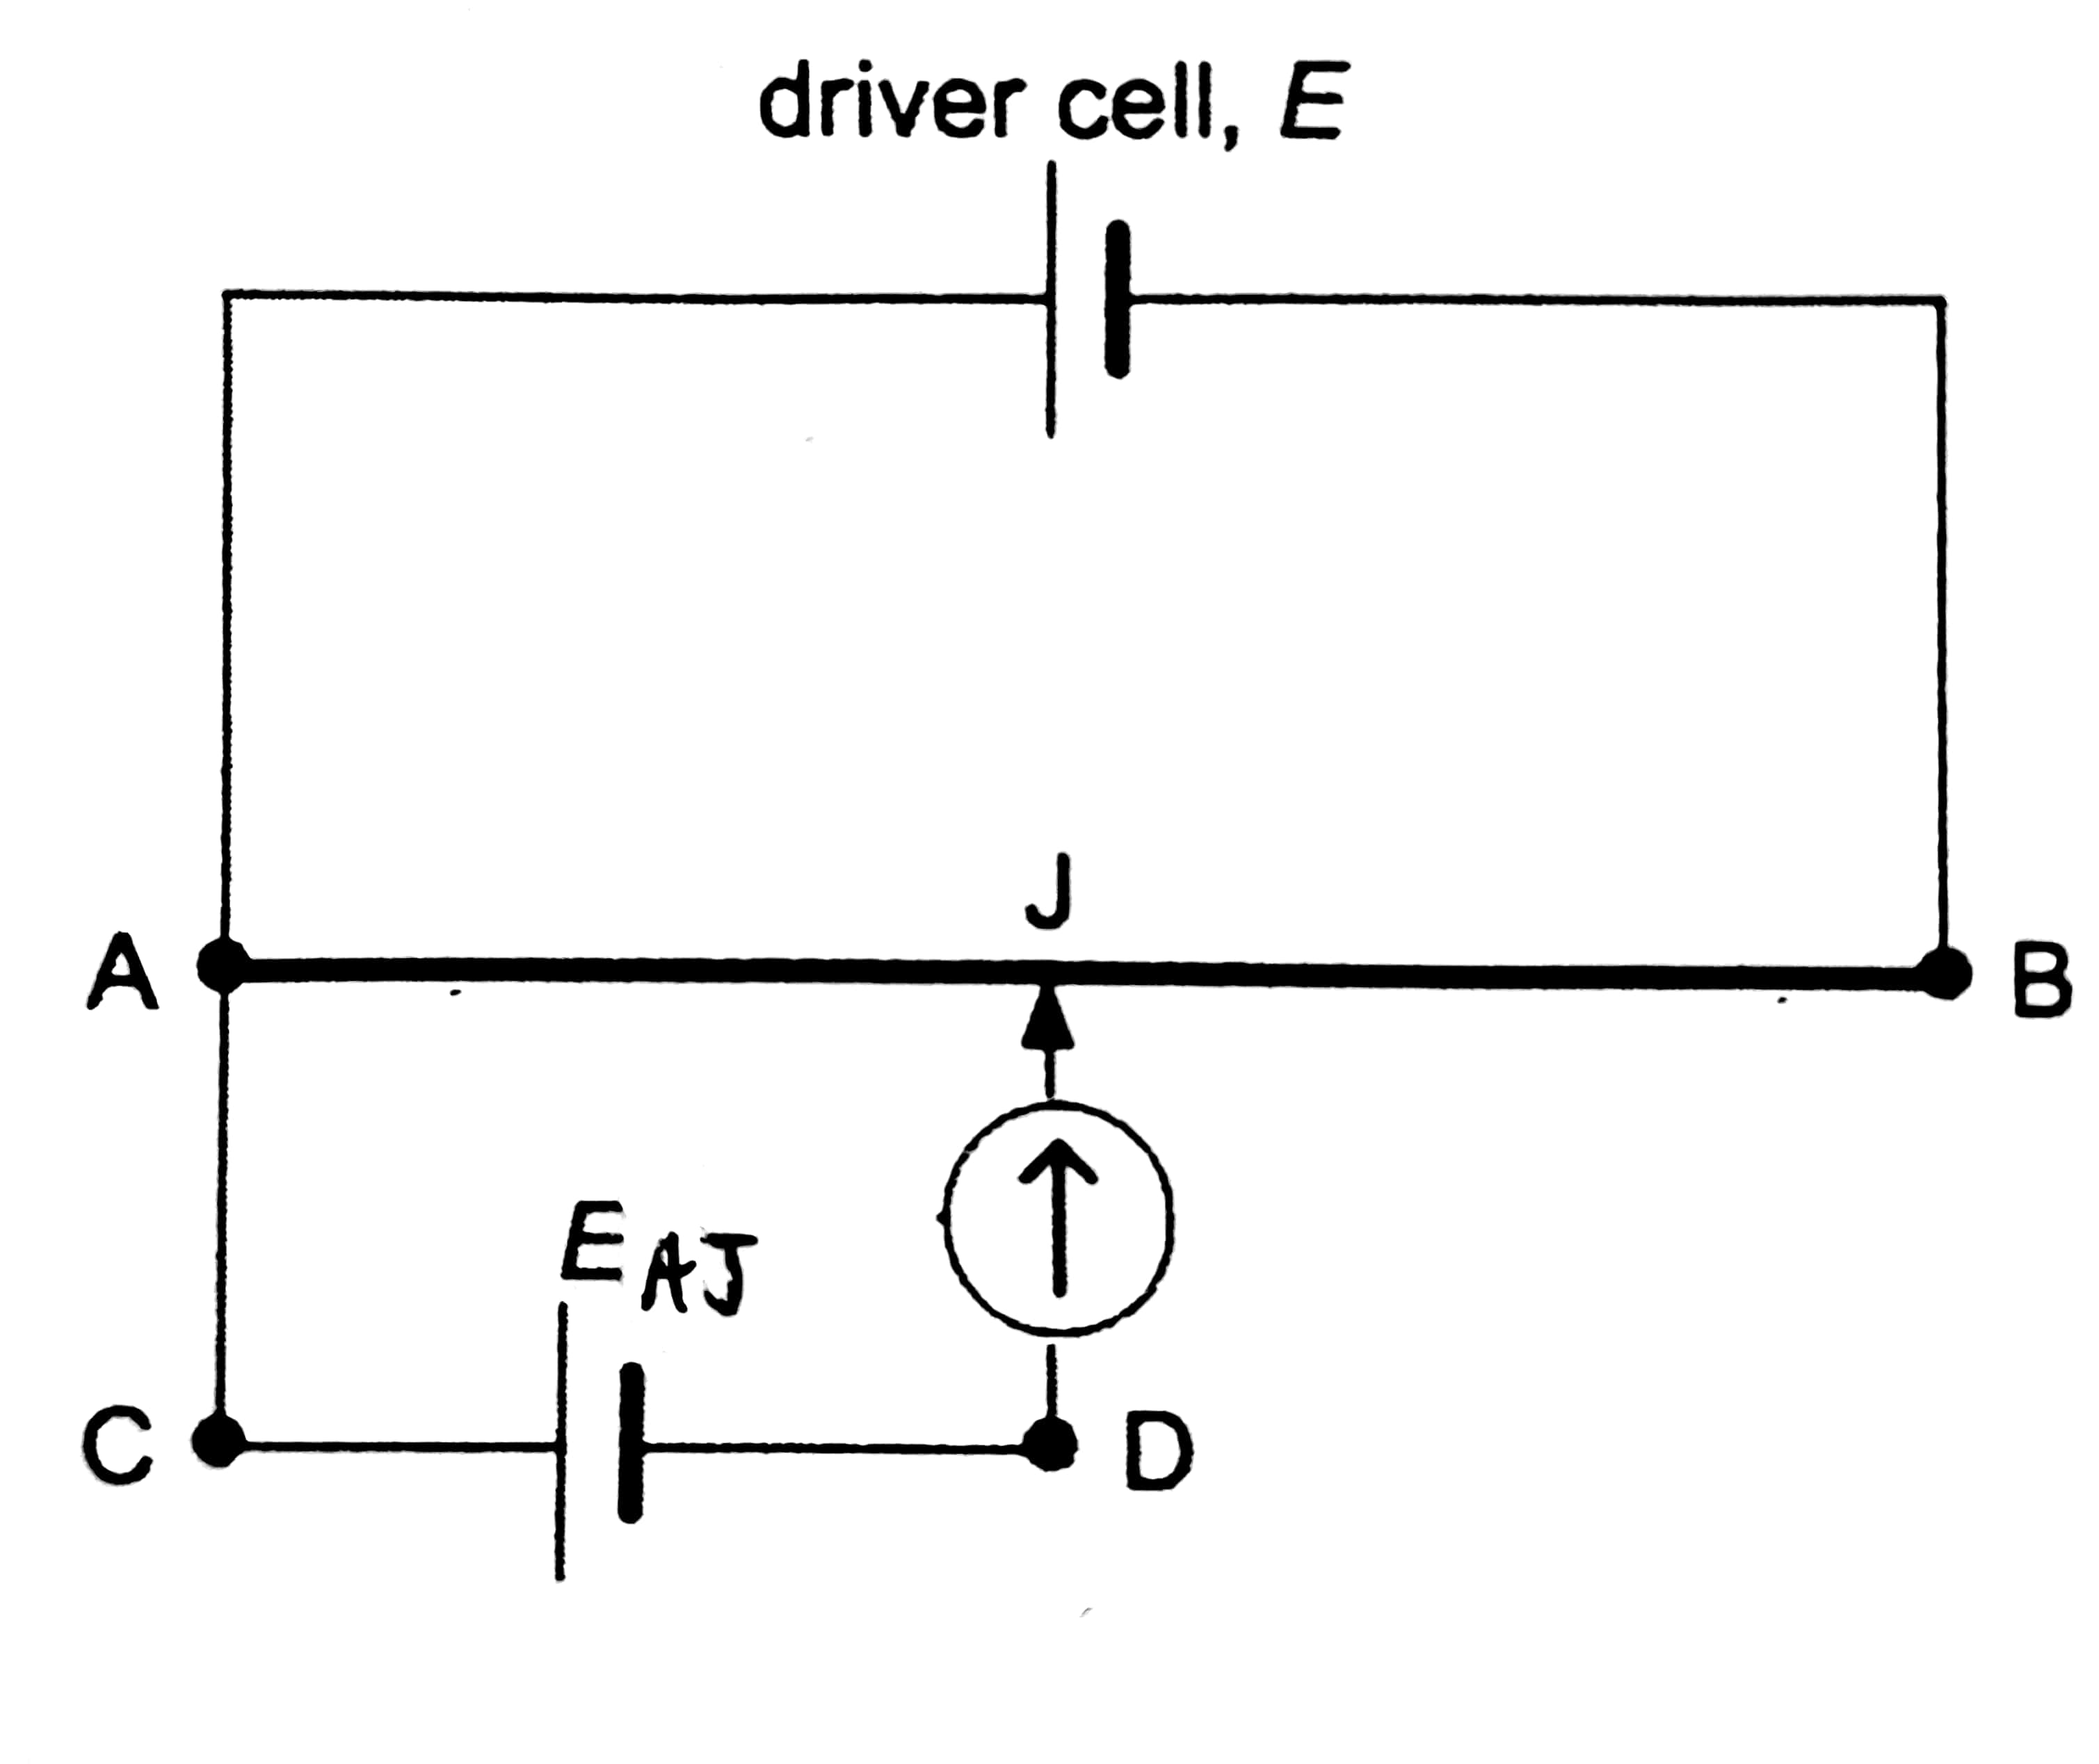
\includegraphics[width=0.4\columnwidth]{../images/DC-Circuits-Potentiometer-1.jpg}
            \captionsetup{type=figure}
            \caption[figure]{\ref{RVHS} An illustration of a potentiometer.}
        \end{center}
        \item In the circuit below, the internal resistance \(r\) satisfies
        \[\frac{L_{AJ_2}}{L_{AJ_1}}=\frac{R}{R+r}.\]
        \begin{center}
            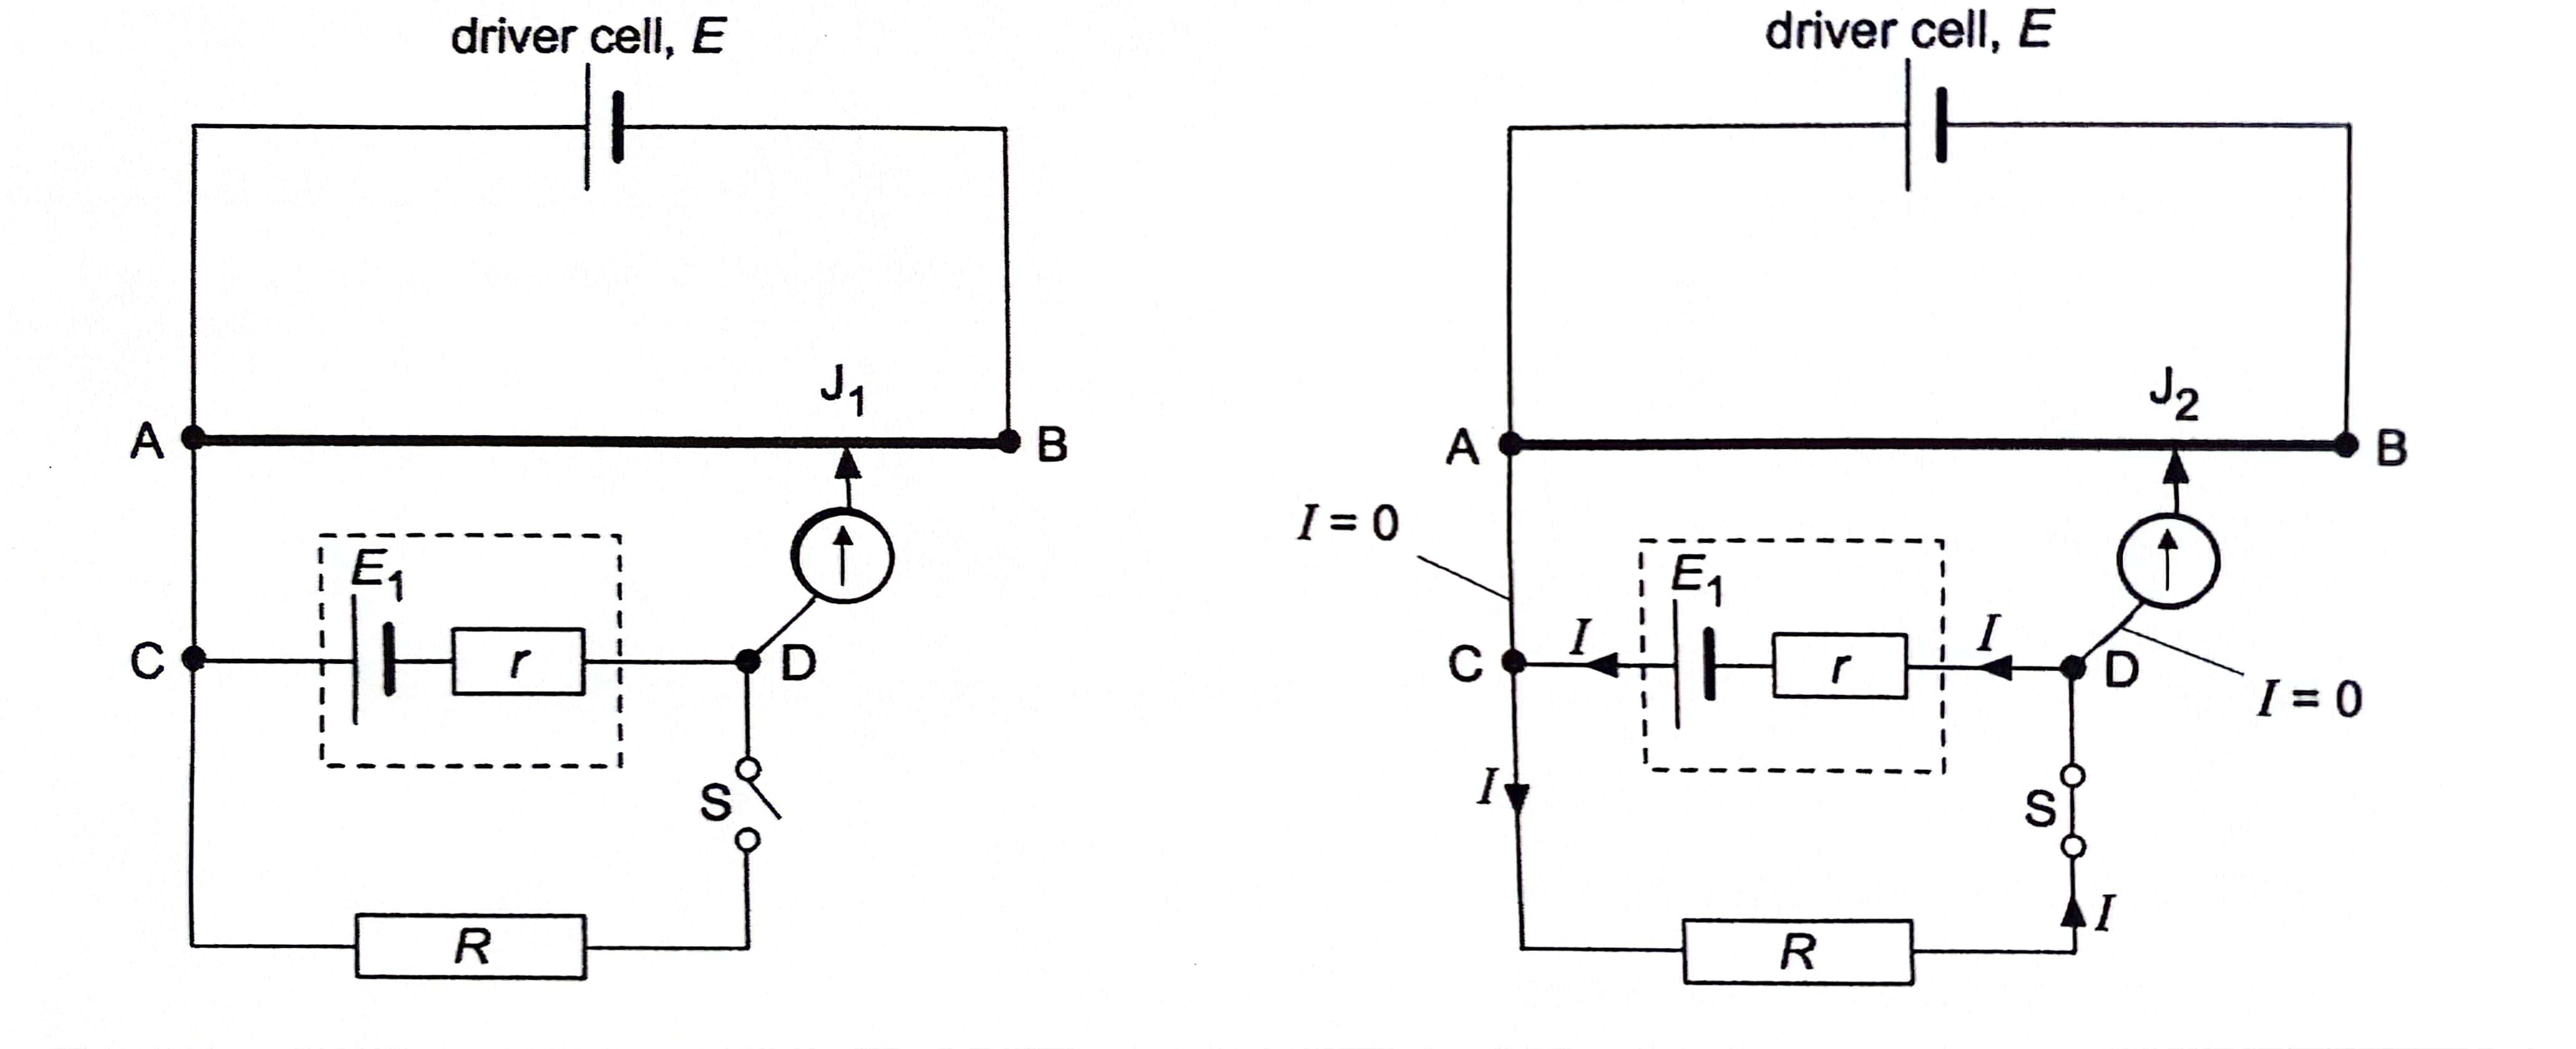
\includegraphics[width=0.88\columnwidth]{../images/DC-Circuits-Potentiometer-2.jpg}
            \captionsetup{type=figure}
            \caption[figure]{\ref{RVHS} Some more illustrations of potentiometers.}
        \end{center}
        For the diagram to the left, why \(V_{CD}=V_{AJ_1}\) is easily seen from the diagram below.
        \begin{center}
            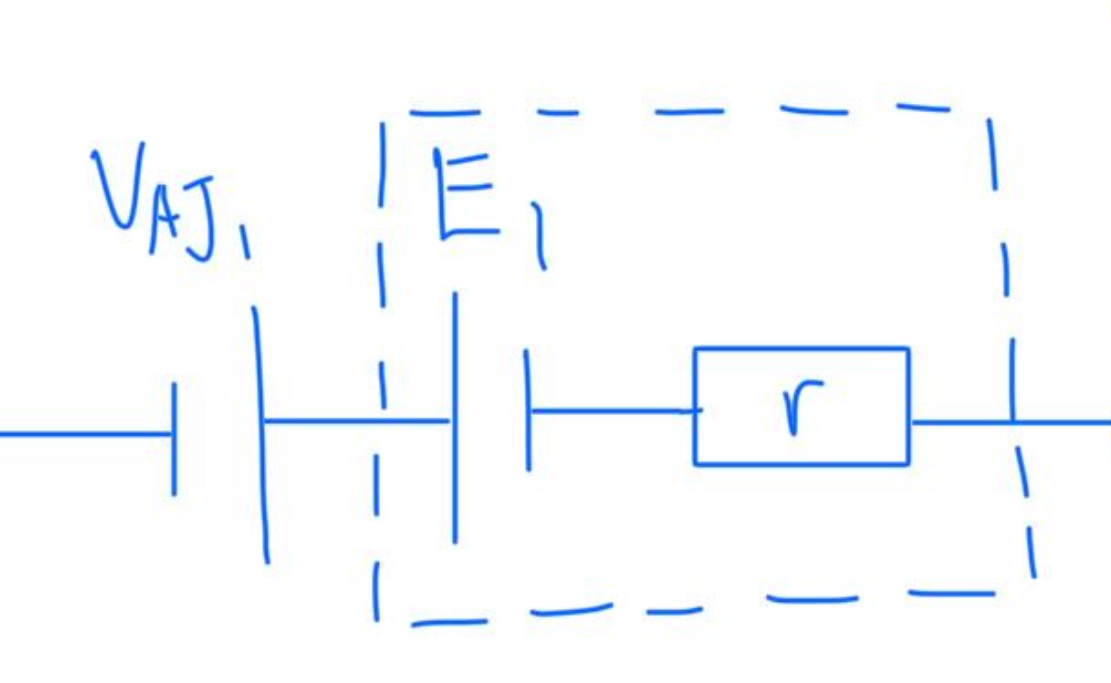
\includegraphics[width=0.3\columnwidth]{../images/D.C.-Voltage-Cancelling-Each-Other.png}
            \captionsetup{type=figure}
            \caption[figure]{\ref{Me} Part CD of the circuit.}
        \end{center}
    \end{itemize}
\end{itemize}

\chapter{Electromagnetism}
\begin{center}
    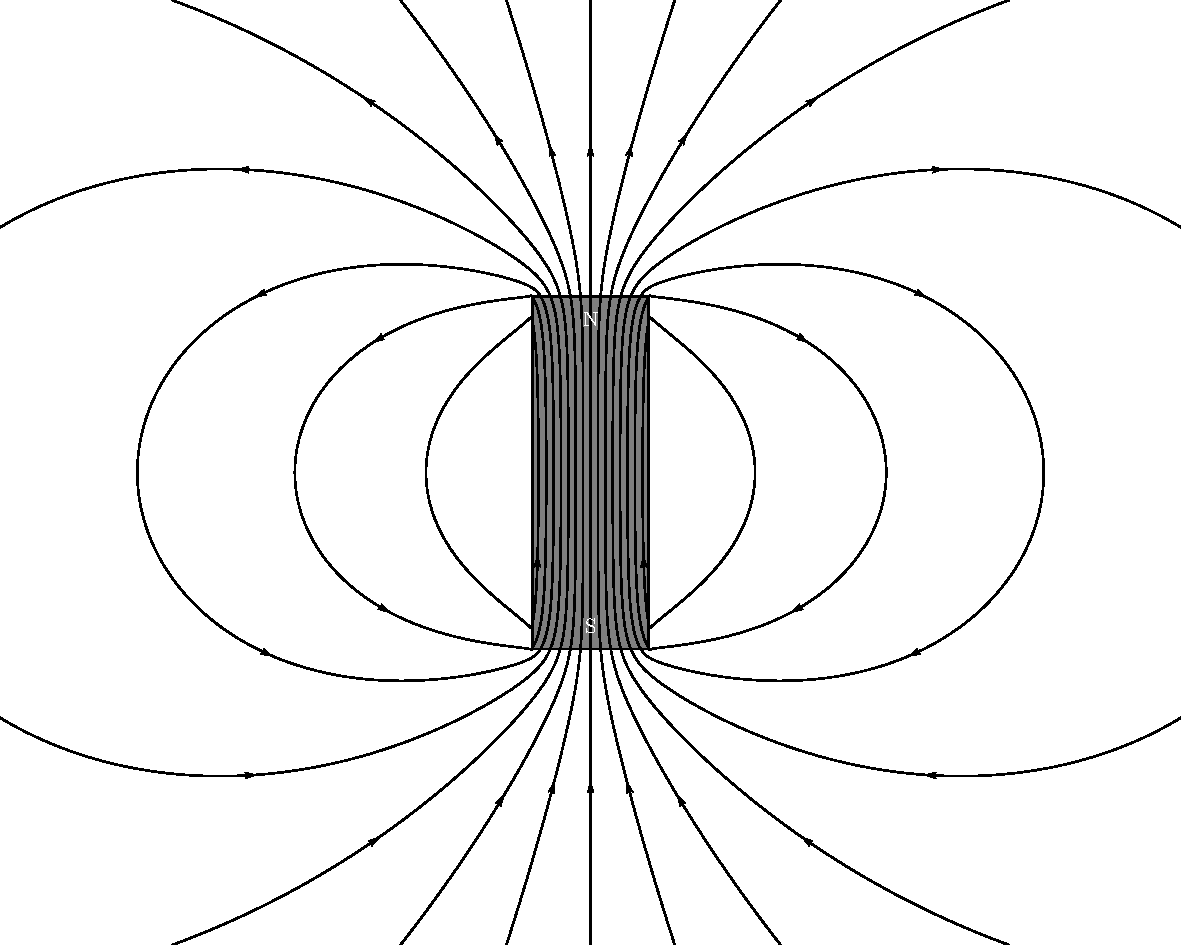
\includegraphics[width=0.8\textwidth]{../images/Bar-Magnet/Bar-Magnet.pdf}
    \captionsetup{type=figure}
    \caption[figure]{\ref{Magnetic field produced by a bar magnet} Magnetic field produced by a bar magnet.}
\end{center}
\begin{itemize}
    \item A \emph{magnetic field} is a \emph{region of space} where a magnetic pole, moving charged particular or current-carrying conductor will \emph{experience a magnetic force}.
    \item \emph{Magnetic flux density} is defined as the \emph{force per unit current per unit length} acting on an \emph{infinitely long current-carrying conductor} placed \emph{perpendicularly} to the magnetic field.
    \item Dots and crosses as indicators of direction:
    \begin{center}
        \begin{tabular}{|Sc|Sc|}
            \hline
            \Large \(\bigotimes\) & Into the page\\
            \hline
            \Large \(\bigodot\) & Out of the page\\
            \hline
        \end{tabular}
    \end{center}
    \item Left and right hand rules:
    \begin{center}
        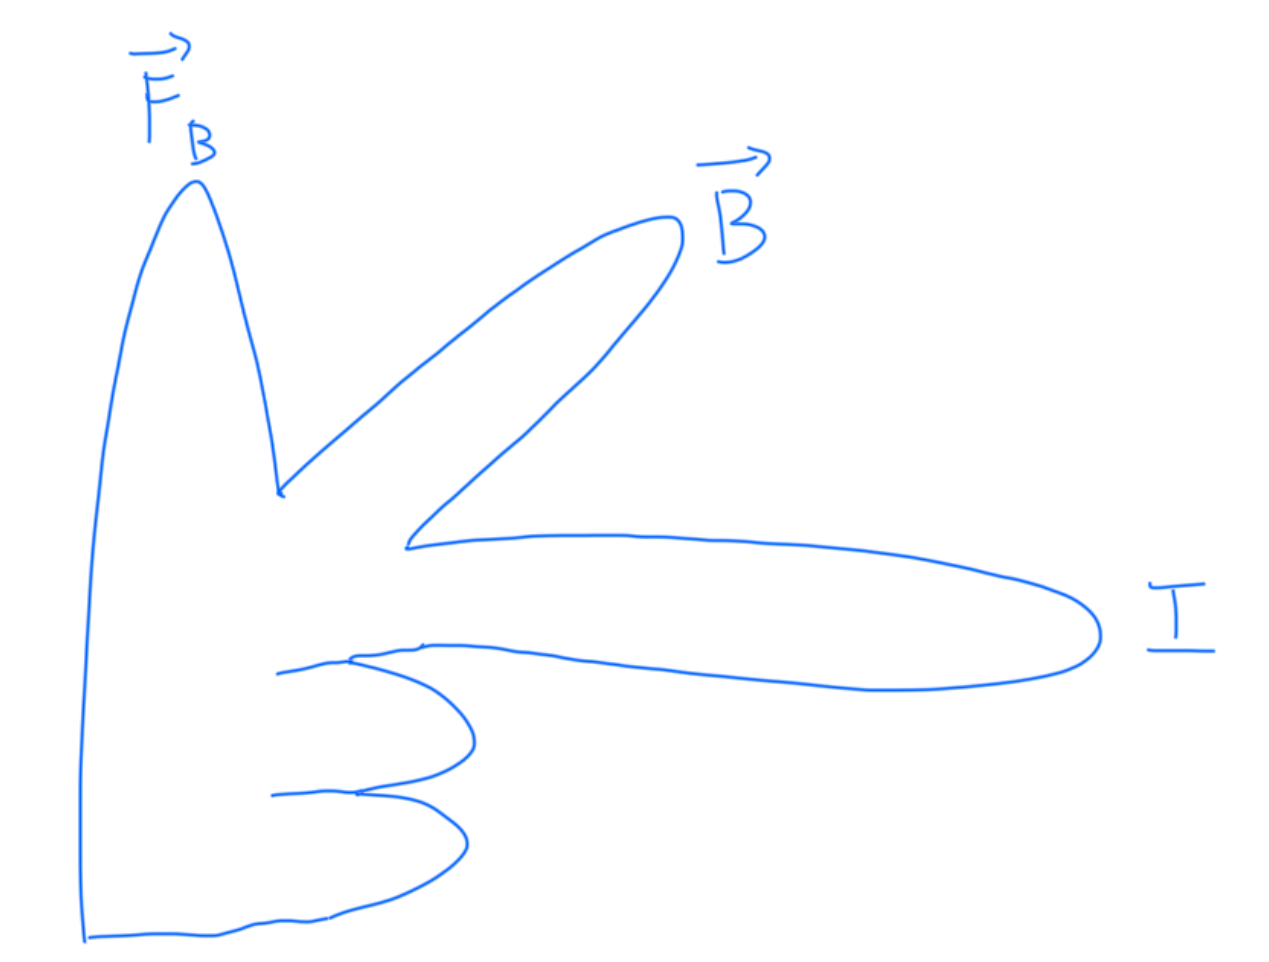
\includegraphics[width=0.5\textwidth]{../images/Left-Right-Hand-Rules/Left-hand-rule.png}
        \hspace{2cm}
        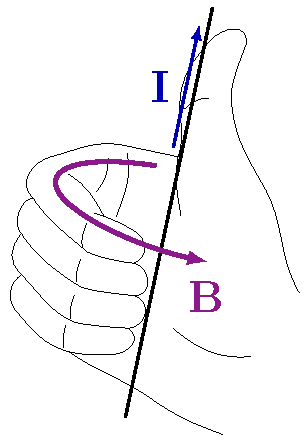
\includegraphics[width=0.28\textwidth]{../images/Left-Right-Hand-Rules/Right-hand-rule.pdf}
        \captionsetup{type=figure}
        \caption[figure]{\ref{Left and right hand rules} Left and right hand rules.}
    \end{center}
    \item At any point some perpendicular distance \(d\) from the center of an \emph{infinitely long straight} current-carrying conductor, the magnitude of the magnetic flux is given by
    \[B=\frac{\mu_0I}{2\pi d}.\]
    Here, \(\mu_0=4\pi\cdot 10^{-7}\) is the permeability of free space.
    \begin{center}
        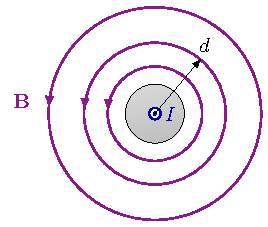
\includegraphics[width=0.5\textwidth]{../images/Current-Carrying-Wire/Current-Carrying-Wire.pdf}
        \captionsetup{type=figure}
        \caption[figure]{\ref{Current in a wire} Current in a wire.}
    \end{center}
    \item At the center of a flat circular coil with \(N\) turns, radius \(r\), and current \(I\) flowing through it, the magnitude of the magnetic flux density is given by 
    \[B=\frac{\mu_0NI}{2r}.\]
    \begin{center}
        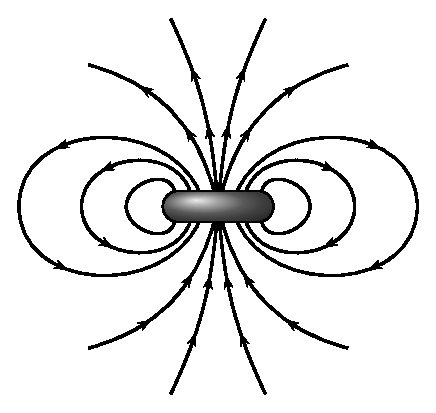
\includegraphics[width=0.5\textwidth]{../images/Flat-Circular-Coil/Flat-Circular-Coil.pdf}        \captionsetup{type=figure}
        \caption[figure]{\ref{Flat circular coil} Current in a flat circular coil.}
    \end{center}
    \item Suppose we have an ideal (having infinite length) solenoid of \(n=N/L\) number of turns per unit length, which has a current \(I\) flowing through it. Then, the magnitude of the uniform magnetic flux density at its center is given by 
    \[B=\mu_0nI.\]
    \begin{center}
        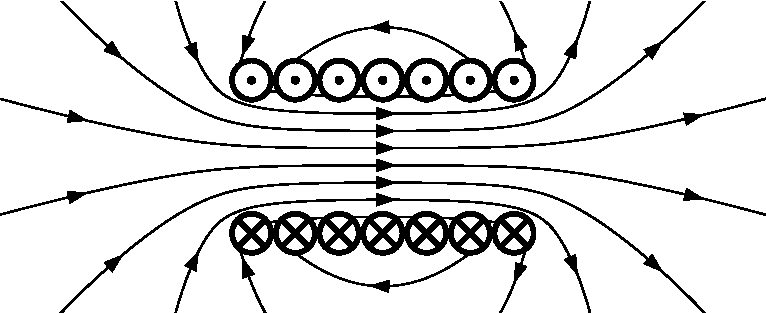
\includegraphics[width=0.9\textwidth]{../images/Solenoid.pdf}
        \captionsetup{type=figure}
        \caption[figure]{\ref{Solenoid} Current in a solenoid and the magnetic field produced.}
    \end{center}
    \item A set of coils can be considered to be a solenoid when the radius of said coils is negligible compared to their length. 
    \item The addition of a ferrous core, of permeability \(\mu\), into a solenoid increases the magnetic flux density there, which is given by 
    \[B=\mu nI.\]
    \item Say we have a straight current-carrying conductor of length \(l\) with current \(I_\perp\) flowing perpendicular to the magnetic field. Then for any point on that conductor that experiences a magnetic flux of density \(B\), 
    \[F_B=BI_\perp l.\]
    \item ~
    \begin{center}
        \begin{tabular}{|Sc|Sc|}
            \hline
            Direction of Current in Two Wires & Direction of Net Magnetic Force\\
            \hline
            Same & Attractive\\
            \hline
            Opposite & Repulsive\\
            \hline
        \end{tabular} 
        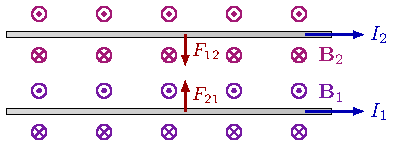
\includegraphics[scale=1.5,page=1]{../images/Two-Current-Carrying-Wires/Two-Current-Carrying-Wires.pdf}

        \includegraphics[scale=1.5,page=2]{../images/Two-Current-Carrying-Wires/Two-Current-Carrying-Wires.pdf}
        \captionsetup{type=figure}
        \caption[figure]{\ref{Two current carrying conductors} Current carrying conductors in parallel.}
    \end{center}
    \item A charge \(q\) moving at speed \(v_\perp\) perpendicular to the magnetic field, of flux density \(B\), experiences a magnetic force of magnitude
    \[F_B=qv_\perp B.\]
    \item Notice that the charged particle above travels in circular motion, with radius and period
    \[r=\frac{mv}{Bq}\qquad\text{and}\qquad T=\frac{2\pi m}{qB}.\]
    \item Velocity selector. Suppose we have a velocity selector with a uniform magnetic field, of flux density \(B\) out of (or into) the paper. Further assume there is an electric field of strength \(E\) rightwards (or leftwards) in the selector. This is illustrated in \hyperlink{Fig-15.7}{Fig 15.7}. Then, for a charged particle perpendicular to both fields to pass (undeflected) through the slits, \(F_E=F_B\). This simplifies to 
    \[v=\frac{E}{B}.\]
    \begin{center}
        \hypertarget{Fig-15.7}{}
        \begin{minipage}{0.9\textwidth}
            \centering
            \raisebox{-0.5\height}{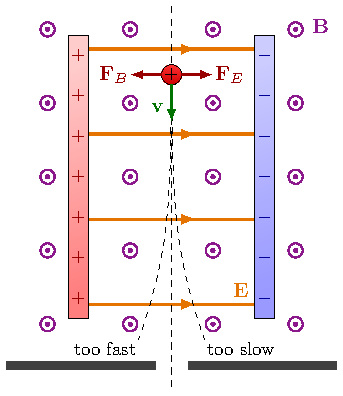
\includegraphics[width=0.45\textwidth,page=1]{../images/Velocity-Selector/Velocity-Selector.pdf}}
            \hspace*{.2in}
            \raisebox{-0.5\height}{\includegraphics[width=0.5\textwidth,page=2]{../images/Velocity-Selector/Velocity-Selector.pdf}}
            \captionsetup{type=figure}
            \caption[figure]{\ref{Velocity selector} An illustration of a velocity selector.}
          \end{minipage}
    \end{center}
\end{itemize}
\newpage
Some nice images:
\begin{center}
    \includegraphics[angle=90,width=\textwidth]{../images/Bar-Magnet/Cropped/1.pdf}
    \includegraphics[angle=90,width=\textwidth]{../images/Bar-Magnet/Cropped/2.pdf}
    \includegraphics[width=0.49\textwidth]{../images/Bar-Magnet/Cropped/3.pdf}
    \includegraphics[width=0.49\textwidth]{../images/Bar-Magnet/Cropped/4.pdf}
    \captionsetup{type=figure}
    \caption[figure]{\ref{Magnetic field produced by a bar magnet} Magnetic fields produced by two bar magnets.}
\end{center}
\chapter{Electromagnetic Induction}
\begin{itemize}
    \item \emph{Magnetic flux} is the \emph{product} of \emph{an area} and the component of \emph{magnetic flux density perpendicular} to that area.
    \item In other words, let \(A\) be an area in a uniform magnetic field, of flux density \(B_\perp\) perpendicular to \(A\). Then, the magnetic flux \(\Phi\) through \(A\) is
    \[\Phi=B_\perp A.\]
    \item The area \(A\) here is a \emph{vector}! When we flip it through \(\pi\) radians, the magnetic flux through it is now \(-\Phi=-B_\perp A\). 
    \item \emph{One weber} is the \emph{magnitude of magnetic flux} through an \emph{area of} \(1\text{m}^2\) when a \emph{magnetic field of} \(1\text{T}\) acts \emph{perpendicularly into} the area.
    \item \emph{Magnetic flux linkage} through a coil is defined as the \emph{product} of the \emph{number of turns} of the coil and the magnetic flux through each turn of the coil.
    \item The magnetic flux through a coil of \(N\) turns is hence
    \[N\Phi=NB_\perp A.\]
    \item \emph{Faraday's Law of Electromagnetic Induction} states that the \emph{e.m.f. induced} in a \emph{conductor} is \emph{directly proportional} to the \emph{rate of change of magnetic flux linkage}.
    \item \emph{Lenz's Law} states that the \emph{direction of the induced e.m.f.} is such that it may produce \emph{an effect} that \emph{opposes the change} causing it.
    \item Lenz's Law is a consequence of conservation of energy. Mechanical work done to enable the change in magnetic flux linkage is converted into electrical energy.
    \item Faraday's and Lenz's Laws imply that the e.m.f generated is
    \[E=-(N\Phi)'=-(NB_\perp A)'.\]
    (The negative sign indicates that the induced e.m.f. opposes the change in magnetic flux linkage.)
    \begin{center}
        \includegraphics[width=0.4\textwidth,page=4]{../images/Lenz's-Law/Lenz's-Law.pdf}
        \includegraphics[width=0.45\textwidth,page=5]{../images/Lenz's-Law/Lenz's-Law.pdf}
        \includegraphics[width=0.4\textwidth,page=3]{../images/Lenz's-Law/Lenz's-Law.pdf}
        \captionsetup{type=figure}
        \caption[figure]{\ref{Lenz's Law} Examples of Lenz's Law in action.}
    \end{center}
    \item Motional e.m.f.: Suppose we have a circuit as shown in the bottom left of the following figure. Then, by Faraday's Law,
    \[\lvert E \rvert=\Phi'=B(\Delta A)=Blv.\]
    \begin{center}
        \begin{minipage}{0.9\textwidth}
            \centering
            \raisebox{-0.5\height}{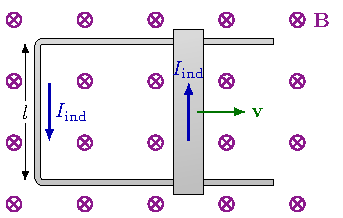
\includegraphics[width=0.58\textwidth,page=1]{../images/Lenz's-Law/Lenz's-Law.pdf}}
            \hspace*{.2in}
            \raisebox{-0.5\height}{\includegraphics[width=0.37\textwidth,page=2]{../images/Lenz's-Law/Lenz's-Law.pdf}}
            \captionsetup{type=figure}
            \caption[figure]{\ref{Lenz's Law} Example of motional emf.}
          \end{minipage}
    \end{center}
    \item Conventions for polarity and when to use them.
    \begin{center}
        \begin{tabular}{|Sc|Sc|Sc|}
            \hline
            Energy conversion & Function in a circuit & Convention for polarity\\
            \hline
            \textcolor{NavyBlue!80}{Electrical} to \textcolor{brown!70}{others} & Resistor/Wire & Higher potential\({}={}\)relatively positive\\
            \hline
            \textcolor{brown!70}{Others} to \textcolor{NavyBlue!80}{electrical} & Battery & Lower potential\({}={}\)relatively positive\\
            \hline
        \end{tabular}
    \end{center}
    \item Faraday's Paradox. Consider a metal disc with of area \(A\) rotating at frequency \(f\) in a uniform magnetic field, of flux density \(B\). Then, let \(\text{O}\) be the centre of the disk, and pick any point \(P\) along the circumference of the disk. We see that \(A'\), the area swept by \(\text{OP}\), is \(\pi r^2f\). So, by Faraday's Law,
    \[E=B\pi r^2f.\]
    \begin{center}
        \includegraphics[width=0.4\textwidth]{../images/Faraday’s-Paradox.png}
        \captionsetup{type=figure}
        \caption[figure]{\ref{Me} An illustration of Faraday's Paradox.}
    \end{center}
\end{itemize}
\chapter{Alternating Current}
\begin{itemize}
    \item An \emph{alternating current (a.c.) source} creates an electrical \emph{current} that varies in magnitude \emph{and} direction \emph{periodically with time}, as opposed to a \emph{direct current} (d.c.) source where the \emph{direction} of the current stays \emph{constant}. 
    \item Alternating current \emph{must change direction}. For instance, the following two functions, namely \(I=sin(t)+1\) and \(I=cos(t)+1\), are both (varying) direct currents.
    \begin{center}
        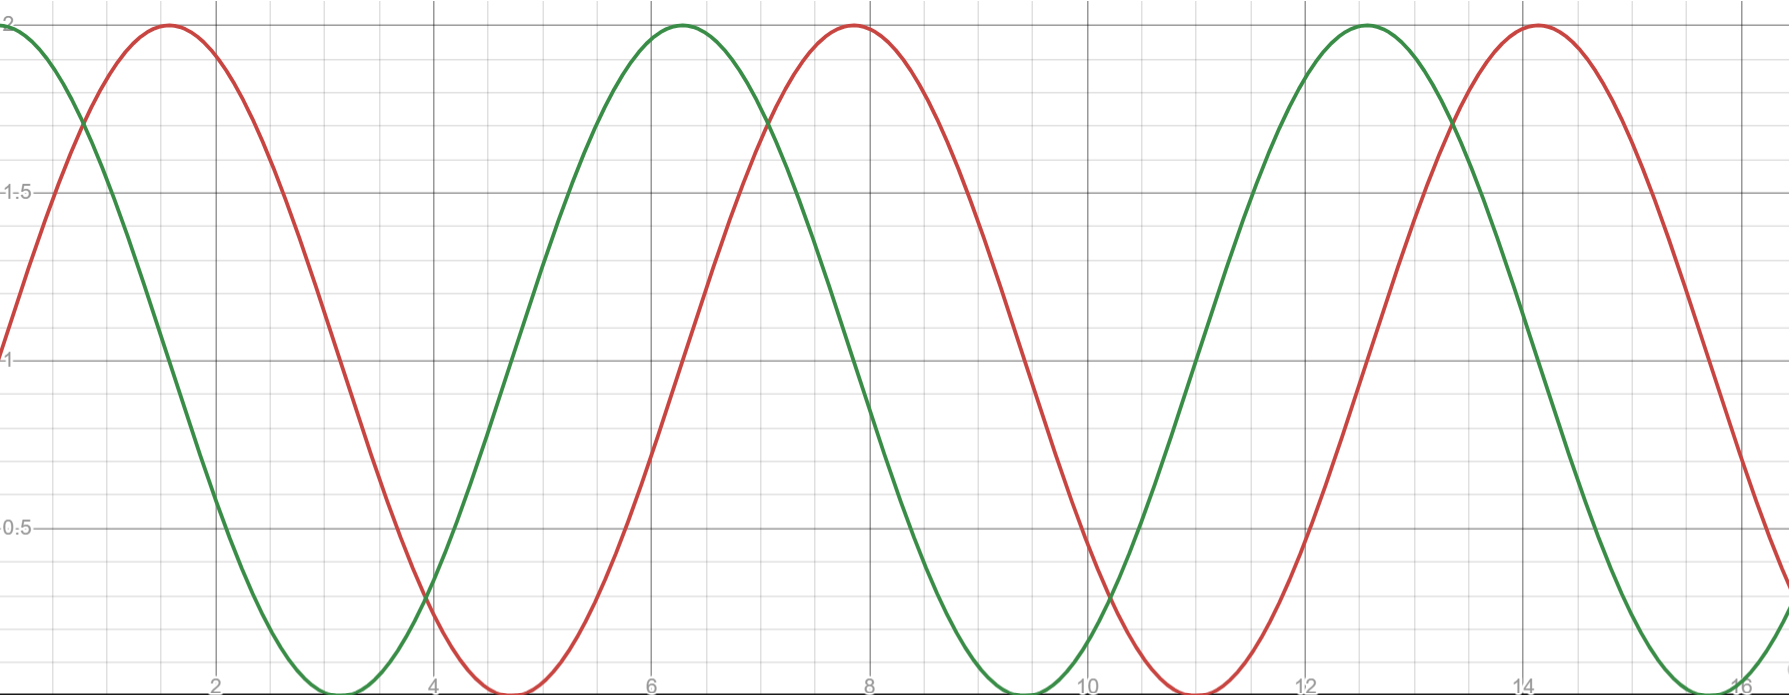
\includegraphics[width=\textwidth-25pt]{../images/Varying-Direct-Current.png}
        \captionsetup{type=figure}
        \caption[figure]{\ref{Varying direct current} Direct currents.}
    \end{center}
    \item The \emph{root-mean-square} (r.m.s.) value \(I_{\text{rms}}\) (or \(V\text{rms}\)) of an \emph{alternating current} (or alternating voltage) is the value of a \emph{steady direct current} (or direct voltage) that would produce the \emph{same average power} in a given resistor.
    \item We denote the mean value of a quantity \(x\) by \(\langle x \rangle\). So, \(x_{rms}=\sqrt{\langle x^2 \rangle}\), and it also holds that
    \[\langle P \rangle=I_\text{rms}^2R=\frac{V_\text{rms}^2}{R}.\]
    \item Steps to determine the rms value: square \(\to\) mean  \(\to\) root.
    \begin{enumerate}
        \item Square all values of \(I\) (or \(V\)).
        \item Find the mean square value \(\langle I^2 \rangle\) (or \(\langle V^2 \rangle\)). This is just the area under the graph of \(I^2\) (or \(V^2\)) against \(t\) in one period.
        \item Square root the value obtained above.
    \end{enumerate}
    \item Note that for a \emph{full wave sinusoidal} alternating current (which an be assumed unless otherwise stated), 
    \[\langle P \rangle=\frac{1}{2}P_0,\qquad V_{\text{rms}}=\frac{1}{\sqrt{2}}V_0,\quad\text{and}\quad I_{\text{rms}}=\frac{1}{\sqrt{2}}I_0.\]
    \item Transformers. Let \(N_P\), \(V_P\), and \(I_P\) be the number of turns, voltage, and current, respectively, in the primary winding. Similarly define \(N_S\), \(V_S\), and \(I_S\) for the secondary winding. Then,
    \[\frac{N_S}{N_P}=\frac{V_S}{V_P}=\frac{I_S}{I_P}.\]
    (To quickly determine which side carries a greater voltage, we can use the principle of `more turns, more voltage'.)
    \item A step up transformer is one that increases voltage, i.e. \(V_S>V_P\) (or \(N_S>N_P\)).
    \item A step down transformer is one that decreases voltage, i.e. \(V_P>V_S\) (or \(N_P>N_S\)).
    \begin{center}
        \includegraphics[width=\textwidth-30pt]{../images/Transformer/TransformerCropped.pdf}
        \captionsetup{type=figure}
        \captionof{figure}{\ref{Transformer} A step-up transformer with \(N_P=40\) and \(N_S=80\).}
    \end{center}
    \begin{center}
        \includegraphics[width=\textwidth-30pt]{../images/Another-Transformer/Another-Transformer.pdf}
        \captionsetup{type=figure}
        \captionof{figure}{\ref{Another Transformer} Another step-up transformers.}
    \end{center}
    \item Transformers cannot be used for \emph{constant} direct current. Since there is no change in voltage/current, no emf will be (constantly) induced in the secondary coil. 
    \item When the direct current varies, however, there will be an \emph{alternating} current induced.
    \item Energy loss in a transformer.
    \begin{enumerate}
        \item Winding resistance. Current flowing through the windings causes \emph{resistive heating} of the conductors.
        \item Hysteresis losses. Each time the \emph{magnetic field is reversed}, a small amount of energy is lost due to hysteresis within the core.
        \item Magnetostriction. Magnetic flux in a ferromagnetic fore causes it to physically expand and contract slightly with each cycle of the magnetic field. This produces a \emph{buzzing sound} and can cause losses due to \emph{frictional heating}.
        \item Mechanical losses. The alternating magnetic field causes fluctuating forces between the primary and secondary windings. These cause vibrations within nearby metalwork, adding to the \emph{buzzing noise} and \emph{consuming a small amount of power}.
    \end{enumerate}
    \item Power is typically transmitted at high voltages to minimise the power lost during transmission.
\end{itemize}
\chapter{Bibliography}
The copyrights belong solely to their respective owners. The images used mostly fall under the CC-BY-SA-3.0 or CC-BY-SA-4.0 licenses. Please contact me if you would like your work removed from these notes, or have you attribution reworked. 
\begin{enumerate}[label={[\arabic*]}]
    \item\label{Projectile motion} Projectile motion \url{https://tug.org/PSTricks/main.cgi?file=Examples/Physics/physics}
    \item\label{Crane} Crane \url{https://tex.stackexchange.com/a/158785}
    \item\label{2024 Eclipse Map} 2024 Eclipse Map \url{https://discord.com/channels/268882317391429632/359052581022203914/1221402243039887451}
    \item\label{Simple harmonic motion} Simple harmonic motion \url{https://tex.stackexchange.com/a/158741}
    \item\label{RVHS} Images from RVHS' notes
    \item\label{Me} Made by me, Grass, in my iPad's native Notes app.
    \item\label{Electric field lines of a point charge} Electric field lines of a point charge \url{https://tikz.net/electric_fieldlines1/}
    \item\label{Electric field lines of two charges} Electric field lines of two charges \url{https://tikz.net/electric_fieldlines2/}
    \item\label{Interaction of a point charge with a charged plate} Interaction of a point charge with a charged plate \url{https://tikz.net/electric_field_image_charge_plane/}
    \item\label{Electric field plots} Electric field plots \url{https://tikz.net/electric_field_plots/}
    \item\label{Electric field lines between parallel plates} Electric field lines between parallel plates \url{https://tex.stackexchange.com/a/488802}
    \item\label{Electron deflection} Electron deflection \url{https://tug.org/PSTricks/main.cgi?file=Examples/Physics/physics}
    \item\label{Magnetic field produced by a bar magnet} Magnetic field produced by a bar magnet \url{https://tex.stackexchange.com/a/470755} 
    \item\label{Current in a wire} Current in a wire \url{https://tikz.net/magnetic_field_wire/}
    \item\label{Left and right hand rules} Left and right hand rules \url{https://tikz.net/righthand_rule/}
    \item\label{Flat circular coil} Flat circular coil \url{https://tex.stackexchange.com/a/523072}
    \item\label{Solenoid} Solenoid \url{https://en.wikipedia.org/wiki/Lenz's_law#/media/File:VFPt_Solenoid_correct2.svg}
    \item\label{Two current carrying conductors} Two current carrying conductors \url{https://tikz.net/magnetic_field_wire_force/}
    \item\label{Velocity selector} Velocity selector \url{https://tikz.net/velocity_selector/}
    \item\label{Lenz's Law} Lenz's Law \url{https://tikz.net/magnetic_field_lenzs_law/}
    \item\label{Varying direct current} Varying direct currents \url{https://www.desmos.com/calculator} (Made by me, Grass.)
    \item\label{Transformer} Transformer \url{https://tex.stackexchange.com/a/158815}
    \item\label{Another Transformer} Another Transformer \url{https://tex.stackexchange.com/a/321965}
\end{enumerate}
\end{document}